\begingroup
\titleformat{\chapter}[block]
{\normalfont\Huge\bfseries\centering} 
{Capítulo \thechapter} 
{0.5em}
{: \LARGE}
[\vspace{1em}\titlerule]

\titlespacing*{\chapter}{0pt}{-60pt}{40pt}

\chapter{Estado del Arte}
\label{cap:2_art}

    En este capítulo explicamos todos los conceptos aparecidos en el proyecto. Mostramos las aplicaciones, tecnologías, herramientas y librerías usadas durante el proceso de desarrollo del mismo, explicando en cada sección las razones y ventajas que tienen sobre otras.

    \section{Generación Aumentada por Recuperación (RAG)}

        La generación aumentada por recuperación o \textbf{RAG} \cite{0003_RAGhowitwork,0003_RAGhowitwork2} por sus siglas en inglés (Retrieval-Augmented Generation), es el concepto principal sobre el que se asienta nuestro proyecto final de máster. Esta técnica complementa la generación de texto que proporcionan los grandes modelos de lenguaje o \textbf{LLMs} (Large Language Models) con información proveniente de datos privados a través de un modelo de recuperación de información, diseñado para buscar en grandes conjuntos de datos o bases de conocimiento. Las respuestas obtenidas de este modo resultan más legibles y más coherentes para el usuario.
        
        \noindent La tecnología RAG ha evolucionado rápidamente en los últimos años, siguiendo distintas etapas ligadas al desarrollo de los grandes modelos de lenguaje (LLM). En sus inicios, surgió junto con la arquitectura \textit{Transformer} y se centró en mejorar los modelos pre-entrenados mediante la incorporación de conocimiento externo. Posteriormente, la aparición de \textit{ChatGPT} marcó un punto de inflexión, al mostrar el potencial del in-context learning y orientar la investigación hacia cómo ofrecer mejor información a los LLM para resolver tareas más complejas y dependientes de conocimiento \cite{gao2024retrievalaugmentedgenerationlargelanguage}.
        
        \noindent Hoy día, la investigación sobre el paradigma RAG continúa evolucionando, tanto que puede ser categorizada en tres etapas \cite{gao2024retrievalaugmentedgenerationlargelanguage} (ver figura \ref{fig:0140_etapasRAG}):
        
        \begin{enumerate}
        	\item \textbf{Naive RAG:} enfoque inicial basado en un esquema tradicional de indexación, recuperación y generación. Es útil, pro presenta problemas de precisión en la recuperación, \textit{alucinaciones} en la generación o redundancia e incoherencia en la integración de información.
        	\item \textbf{Advanced RAG:} surge para intentar superar las limitaciones de la etapa anterior, mejorando tanto indexación (segmentación fina, uso de metadatos, ...) como la post-recuperación (\textit{reranking}). Así reducimos la sobrecarga de información que la damos al LLM y aumentamos la relevancia de esta.
        	\item \textbf{Modular RAG:} representa la etapa más flexible y avanzada. Introduce nuevos módulos y patrones. \textbf{Nota:} esta modalidad no ha investigado en este trabajo.
        \end{enumerate}
        
        \begin{figure}[H]
        	\centering
        	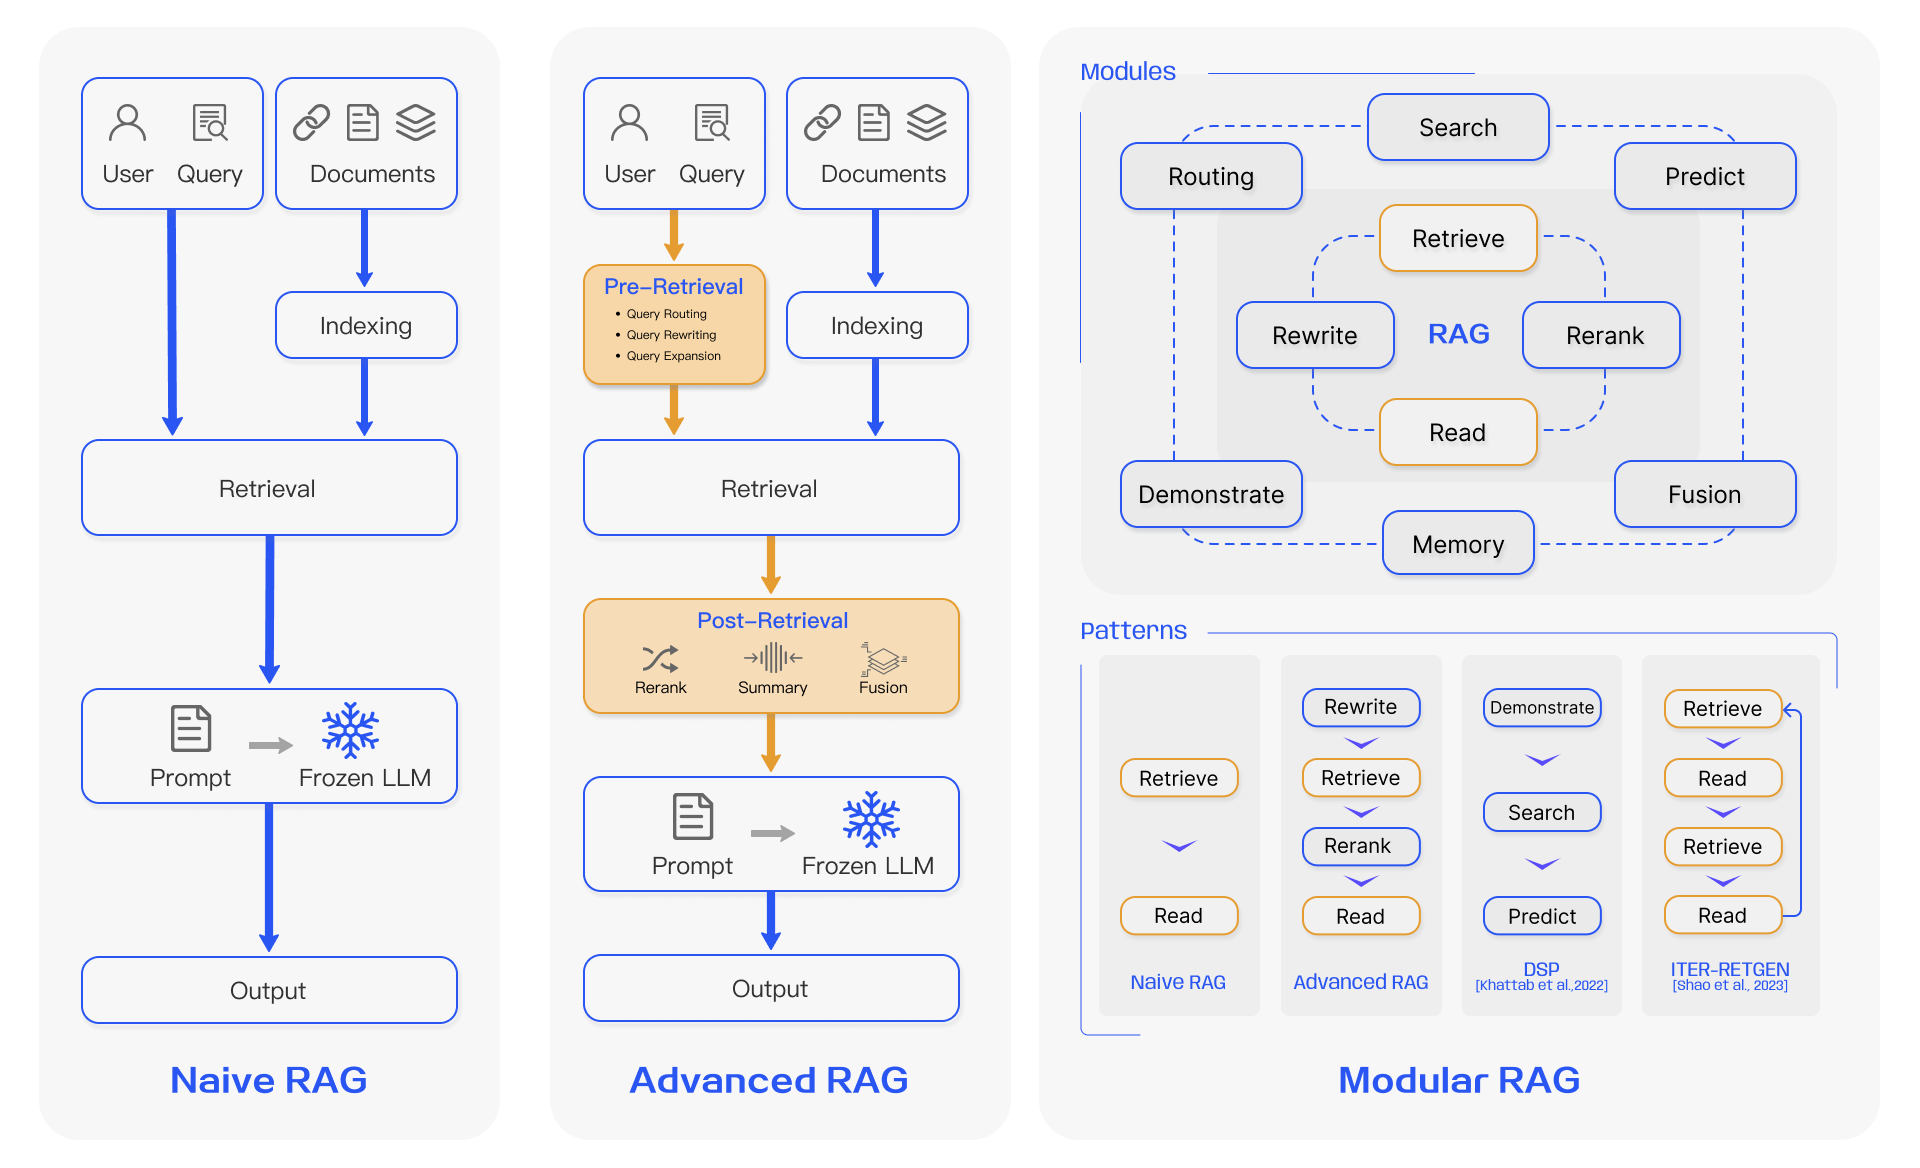
\includegraphics[width=1\textwidth]{imagenes/0140_etapasRAG.png}
        	\caption{Comparación entre los tres paradigma más utilizados de RAG \cite{gao2024retrievalaugmentedgenerationlargelanguage}}		
        	\label{fig:0140_etapasRAG}
        \end{figure} 
        
        \noindent En las siguientes secciones de este apartado iremos desgranando poco a poco más información sobre los conceptos clave LLM-RAG, centrándonos especialmente en el objeto protagonista de este proyecto, el RAG. Mostraremos en que mejora a los LLMs clásicos, explicaremos su funcionamiento y observaremos las ventajas y limitaciones que posee.

        \subsection{Diferencia con los LLMs clásicos}

            Los LLMs tradicionales, como GPT-3 o GPT-4, son modelos pre-entrenados o PLMs (sección \ref{sec:evo_llm}) con grandes conjuntos de datos que generan texto de acuerdo a la información contenida en esos datos \cite{0001_compRAGLLM}. Por lo tanto, su conocimiento esta limitado a la fecha en que fue entrenado, y puede generar respuestas genéricas, no precisas o directamente desfasadas. A este fenómeno se le conoce como \textit{LLM hallucinations} o alucinaciones \cite{0002_LLMhallu}.

            \noindent Optimizar estos modelos para que contengan la información más actualizada y reciente requiere de realizar re-entrenos constantemente, lo que consume muchos recursos y tiempo, por lo que no es una solución adecuada.

            \noindent Los sistemas RAG usan datos recuperados en tiempo real de bases de datos externas en el momento de generar su respuesta al usuario. De esta forma el RAG esta provisto de datos recientes y específicos para el contexto del usuario, sin la necesidad de re-entrenar ningún modelo. La figura \ref{fig:0001-llm-rag} muestra de forma básica este comportamiento.

            \begin{figure}[H]
            	\centering
            	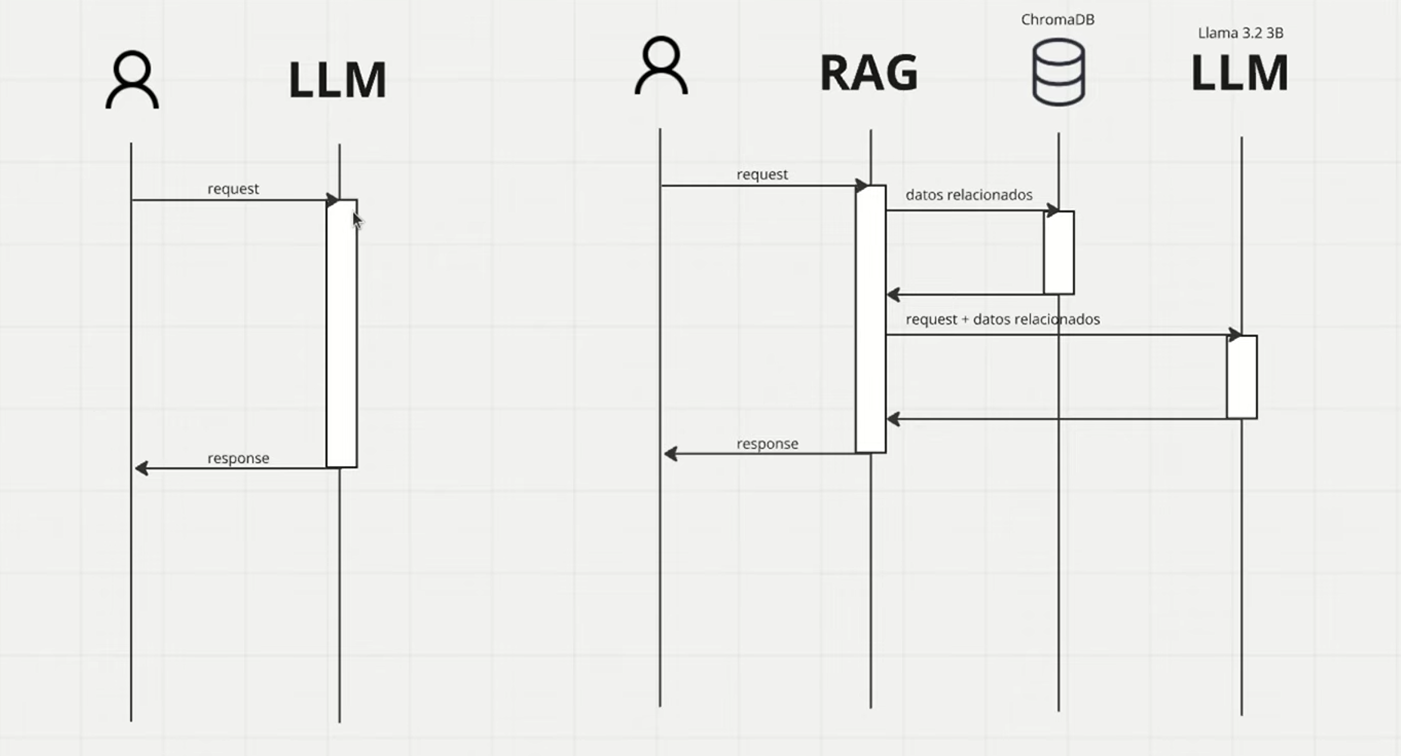
\includegraphics[width=0.8\textwidth]{imagenes/0001-llm_rag.png}
            	\caption{Diferencia básica entre el mecanismo de respuesta de LLM y de RAG. Los LLM responden usando los datos con los que han sido entrenados, mientras que el RAG accede a una base de datos para responder con datos más específicos}		
            	\label{fig:0001-llm-rag}
            \end{figure}  

            \noindent Esta diferencia ayuda al modelo de lenguaje usado por el RAG a adaptar su respuesta al contexto propio del usuario, aportando información relevante y actualizada a la que los LLMs de uso general no tienen acceso.

            \noindent
            
        \subsection{¿Como funciona un RAG?}

            Un sistema RAG se puede comprender como un guión en el que hay que seguir unos pasos para conseguir una respuesta contextualizada y coherente para el usuario \cite{0003_RAGhowitwork,0003_RAGhowitwork2,gao2024retrievalaugmentedgenerationlargelanguage}. Estos pasos se pueden englobar en tres etapas claramente diferenciadas en el proceso de funcionamiento de un RAG, y son las siguientes:

            \subsubsection{Creación del Vector Store}

                El Vector Store es la base de datos que almacenará todo el conocimiento necesario para la lógica de negocio del sistema RAG. Los pasos dentro de esta etapa se pueden resumir en tres: conseguir un conjunto de datos, trocear o separar los datos y almacenar los datos usando modelos de embedding.

                \noindent El conjunto de datos para el RAG es esencial, puesto que en él se reúnen los datos específicos y contextuales que necesitamos y que no poseen los LLMs genéricos. En la mayoría de casos de uso, la información requerida esta contenida en manuales, bases de datos de productos o listas de preguntas frecuentes \cite{0003_RAGhowitwork}.

                \noindent El troceado de datos es el proceso en el cual los datos son transformados en piezas más pequeñas y a su vez más manejables, por ejemplo, dividir un documento de 100 páginas en partes más pequeñas puede ayudar a responder más preguntas a los usuarios. Esto también incrementa la eficiencia del RAG, puesto que el sistema puede obtener rápidamente los trozos de información más relevantes en vez procesar un documento entero.

                \noindent Por último, una vez troceados los datos, necesitamos almacenarlos en nuestra base de datos convertidos en representaciones vectoriales. Esto requiere del uso de los modelos de embedding (sección \ref{sec:embeddings}), que son modelos de lenguaje que transforman el texto de los datos en representaciones numéricas, capturando en ellas las relaciones semánticas del texto durante el proceso (ver figura \ref{fig:0002-rag-db}).

                \begin{figure}[H]
                	\centering
                	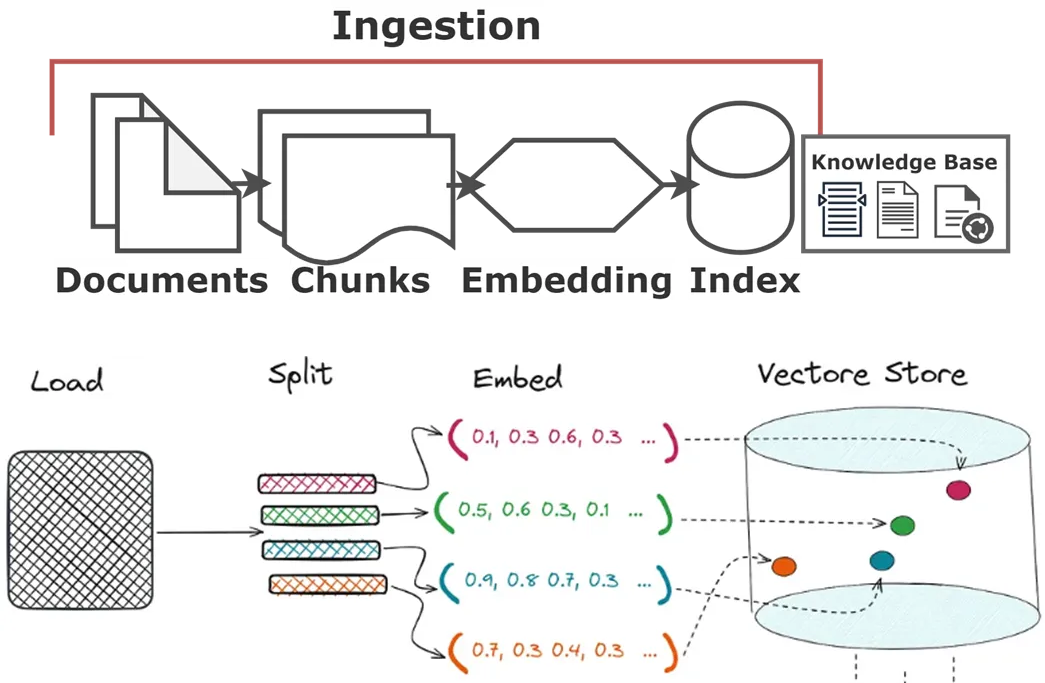
\includegraphics[width=0.6\textwidth]{imagenes/0002-rag-db.png}
                	\caption{Proceso de creación del Vector Store. Se observa todo el proceso: carga, troceado, embedding y almacenamiento \cite{0004_RAGarch}}		
                	\label{fig:0002-rag-db}
                \end{figure}  

            \subsubsection{Recuperación de información}      

                La recuperación de información es la etapa donde entra una consulta al sistema RAG, esta debe ser también vectorizada usando los mismos modelos de embedding que los usados al crear la Vector Store, para garantizar la uniformidad en la respuesta.

                \noindent Una vez vectorizada la consulta el sistema compara ambos embeddings, identifica y retorna las piezas de documentos más parecidas usando medidas de comparación como la similaridad coseno o distancia euclídea entre otras \cite{0003_RAGhowitwork}.La figura \ref{fig:0003-rag-in-action} muestra parte de este proceso.

                \begin{figure}[H]
                    \centering
                    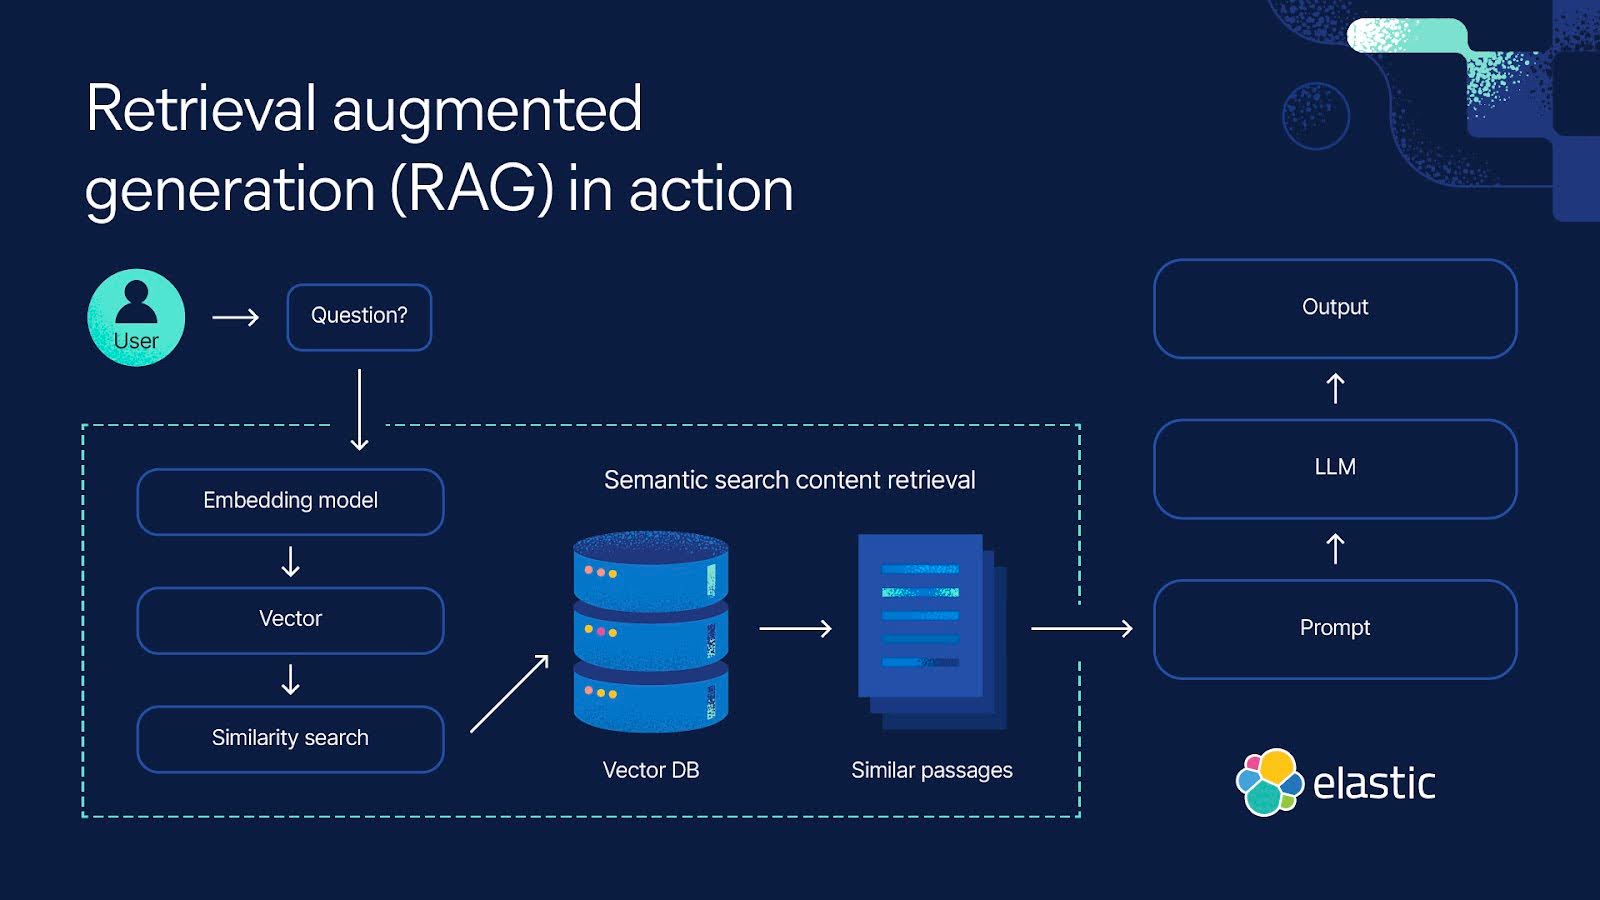
\includegraphics[width=0.8\textwidth]{imagenes/0003-rag-in-action.jpeg}
                    \caption{Fases del proceso de funcionamiento de RAG, se observan las fases de recuperación de información y generación \cite{0003_RAGhowitwork2}}
                    \label{fig:0003-rag-in-action}
                \end{figure}

            \subsubsection{Generación}

                La generación es la etapa que siempre sigue a la recuperación de información. Los documentos recuperados de la consulta inicial son aportados al LLM a través de un prompt \cite{0003_RAGhowitwork2}, que ayuda a generar mediante una serie de instrucciones una respuesta coherente. En la figura \ref{fig:0003-rag-in-action} se puede ver parte de este proceso.

                \noindent Las respuestas obtenidas de esta forma son, en general, más precisas y relevantes dado el contexto, puesto que han sido generadas a partir de los documentos recuperados más relevantes de la base de conocimiento que posee el RAG.
                
        \subsection{Beneficios del RAG}
                       
            Un sistema RAG ofrece múltiples ventajas frente a los modelos de lenguaje que operan de manera aislada. Uno de los principales beneficios es que permite al modelo acceder a información actualizada mediante la integración de fuentes externas, lo que garantiza que las respuestas generadas sean recientes y relevantes para el usuario \cite{0003_RAGhowitwork2}. Esta capacidad de actualización continua resulta clave en entornos donde el conocimiento cambian o evolucionan rápidamente.
                    
            \noindent Otro aspecto destacable es la eficiencia en términos de recursos. Los sistemas basados en RAG suelen requerir menos capacidad de cómputo y almacenamiento, lo que los convierte en una opción más rentable para muchas aplicaciones. Además, al basarse en documentos recuperados durante la consulta, un RAG puede citar sus fuentes y proporcionarlas al usuario, lo que aumenta la transparencia y permite verificar la precisión de las respuestas ofrecidas.
                    
             \noindent En cuanto a la personalización, aunque los modelos de lenguaje ya permiten generar respuestas adaptadas, los RAG va un paso más allá al incorporar mecanismos de recuperación semántica. Esto le permite referenciar contenidos relevantes a partir del contexto específico de la consulta, mejorando la calidad y precisión de las respuestas. Asimismo, frente a preguntas complejas o ambiguas, donde un modelo tradicional podría generar respuestas erróneas o alucinaciones \cite{0002_LLMhallu}, un RAG se apoya en evidencia externa, lo que reduce significativamente este riesgo.
                    
            \noindent Por último, los modelos RAG son altamente versátiles y pueden aplicarse a una amplia gama de tareas de procesamiento de lenguaje natural, como sistemas conversacionales, generación de contenido o recuperación de información, consolidándose así como una herramienta poderosa en el desarrollo de soluciones basadas en inteligencia artificial \cite{0003_RAGhowitwork2}.
        
        \subsection{Desafíos y limitaciones de RAG}
        
            Si bien los sistemas RAG ofrecen ventajas significativas frente a los modelos de lenguaje que operan de forma aislada, también presenta diversos desafíos y limitaciones que deben ser considerados. Uno de los más relevantes es la posibilidad de recuperar información incorrecta o no confiable. Dado que un RAG se basa en fuentes externas para elaborar sus respuestas, una recuperación inadecuada puede derivar en resultados imprecisos o incluso engañosos, afectando la calidad general del sistema.
                    
            \noindent Otro aspecto crítico es el tiempo de búsqueda \cite{0003_RAGhowitwork2}. Al requerir consultas en grandes bases de conocimiento o incluso en la web, el proceso de recuperación puede introducir una latencia considerable, lo que impacta en la experiencia del usuario y en la eficiencia del sistema. Esta limitación exige estrategias de optimización tanto en la indexación como en el diseño de los mecanismos de búsqueda.
                    
            \noindent Además, integrar recuperación y generación en una misma aplicación supone retos importantes en cuanto a diseño e implementación. Es necesario desarrollar soluciones cuidadosas, lo cual puede dificultar la capacitación de los modelos y aumentar la complejidad técnica.
                    
            \noindent La privacidad representa otro desafío relevante \cite{0003_RAGhowitwork2}, especialmente cuando un RAG opera con datos sensibles o confidenciales. En estos casos, es fundamental garantizar el cumplimiento de normativas y políticas de protección de datos, lo que a su vez puede restringir el conjunto de fuentes disponibles.
                    
            \noindent Finalmente, cabe destacar que, por su naturaleza centrada en la recuperación de hechos verificables, un RAG puede mostrar limitaciones a la hora de generar contenido imaginativo o creativo \cite{0003_RAGhowitwork2}. Aunque esto no representa un inconveniente para tareas centradas en la precisión, sí puede reducir su efectividad en aplicaciones donde se espera una mayor capacidad de invención.
        
        \subsection{Tendencias futuras de RAG}
    
            En cuanto al futuro de la generación aumentada por recuperación, las tendencias indican que las tecnologías empleadas para su desarrollo serán cada vez más eficientes y adaptables a una amplia variedad de aplicaciones.
            
            \noindent Los modelos RAG seguirán avanzando hacia una mayor personalización \cite{0003_RAGhowitwork2}, integrando conocimientos específicos del usuario para ofrecer respuestas más precisas y relevantes. Esto será especialmente útil en sistemas de recomendación de contenido y asistentes virtuales, donde la adaptación al perfil del usuario es clave. Además de la personalización, se espera que los usuarios adquieran un mayor control sobre el comportamiento de los modelos, con opciones para ajustar estrategias de búsqueda o modificar la estructura y segmentación del contenido de las bases de datos utilizadas durante la recuperación de información.
            
            \noindent Otra tendencia relevante es el crecimiento en la escalabilidad de los modelos RAG \cite{0003_RAGhowitwork2}, lo que les permitirá manejar un volumen cada vez mayor de datos e interacciones sin comprometer el rendimiento. Asimismo, la integración de RAG con otras técnicas de inteligencia artificial —como el aprendizaje por refuerzo— promete sistemas más versátiles y sensibles al contexto, capaces de gestionar distintos tipos de datos y tareas de forma simultánea.
            
            \noindent Finalmente, a medida que los modelos RAG mejoren en velocidad de recuperación y generación de respuestas \cite{0003_RAGhowitwork2}, será más común su implementación en aplicaciones que demandan baja latencia y tiempos de respuesta en tiempo real, ampliando así su presencia en cualquier entorno.

    \section{Evolución de los LLMs hasta nuestros días}
    \label{sec:evo_llm}

        La forma de extraer información de fuentes de datos textuales ha cambiado ostensiblemente en la última década. Como término, el procesamiento del lenguaje natural ha sobrepasado a la minería de datos como aspecto más importante. Uno de los principales  motivos de este cambio fue la aparición de los modelos de lenguaje, que son utilizados como base para multitud de aplicaciones dedicadas a extraer información valiosa de texto en crudo.

        \noindent Los modelos de lenguaje usan técnicas de aprendizaje automático para predecir palabras mediante probabilidades. Estos modelos aprenden a través de conjuntos de datos textuales, y suelen ser usados para producir textos originales, el reconocimiento de discursos, el reconocimiento óptico de caracteres o el reconocimiento de escritura a mano \cite{0005_journeyLLM,zhao2025surveylargelanguagemodels}.
    
        \noindent La evolución de los modelos de lenguaje ha pasado por cuatro etapas diferenciadas como se pueden observar en la figura \ref{fig:0004-lm-evo}. A continuación, describiremos brevemente estas:
        
        \begin{figure}[H]
            \centering
            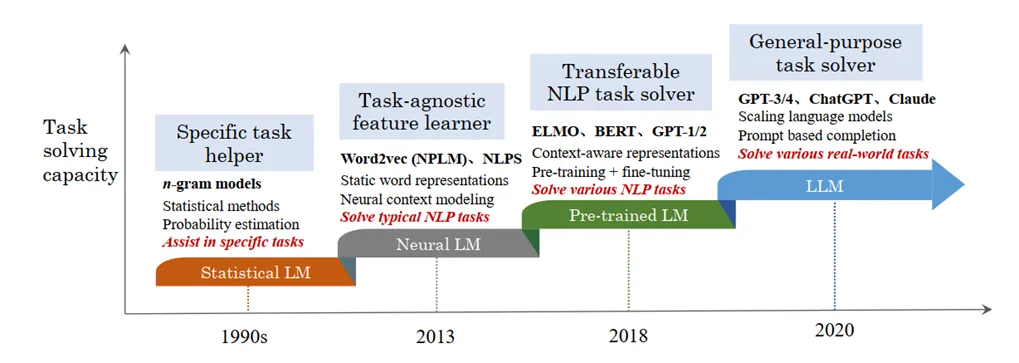
\includegraphics[width=1\textwidth]{imagenes/0004-lm-evo.png}
            \caption{Gráfica de las cuatro etapas en la evolución de los modelos de lenguaje \cite{zhao2025surveylargelanguagemodels}}
            \label{fig:0004-lm-evo}
        \end{figure}
    
        \subsubsection{Modelos de lenguaje estadísticos (SLMs)}
        
            Los modelos de lenguaje estadísticos o SMLs surgieron a partir de el año 1990, e intentaban adivinar la siguiente palabra basándose en las palabras que la precedían. Estos modelos son llamados n-gramas \cite{0005_journeyLLM}: por ejemplo, los bigramas y trigramas predicen según las dos y las tres palabras anteriores respectivamente.
            
            \noindent Mientras los SMLs eran buenos para tareas como la búsqueda de información y la comprensión del lenguaje, tenían un gran inconveniente: la predicción basada en muchas palabras previas, los llamados modelos de gran orden, se complicaba en demasía. La razón principal era la necesidad de estimar un valor exponencial de probabilidades de transición, que en resumen, son valores numéricos comprendidos entre 0 y 1 que representan la probabilidad de que una palabra específica (B) aparezca tras una palabra (A) en una secuencia. 
        
        \subsubsection{Modelos de lenguaje neuronales (NLMs)}
        
            Los SLMs eran buenos al predecir el orden de las palabras, pero fallaban a la hora de entender el lenguaje en profundidad. Los nuevos modelos llamados modelos de lenguaje neuronales o NLMs \cite{0005_journeyLLM} usaban herramientas potentes como redes neuronales, por ejemplo el MLPs (perceptron multicapa) y RNNs (redes neuronales recursivas), que capturaban las relaciones entre palabras. Las modelos como \textit{word2vec} \cite{zhao2025surveylargelanguagemodels} creaban representaciones vectoriales (también denominado modelo de \textit{embeddings}) para cada palabra, ayudando así a a la comprensión de la red de la idea general. 
            
            \noindent Este pequeño avance hacia la compresión del significado de las palabras, no sólo el orden, ha revolucionado como los sistemas procesan el lenguaje, permitiendo a su vez ampliar el rango de tareas en el que son más efectivos, como la generación de texto o la traducción automática de idiomas. Más información sobre modelos de embedding en la sección \ref{sec:embeddings} de esta memoria.
            
        \subsubsection{Modelos de lenguaje pre-entrenados (PLMs)}
        
            Los modelos de lenguaje pre-entrenados o PLMs \cite{0005_journeyLLM}, son modelos que han sido entrenados con un conjunto de datos a través de técnicas de aprendizaje no supervisado. Durante la etapa de pre-entrenamiento, el modelo aprende a comprender y generar texto natural mediante el procesado de grandes cantidades de texto; como por ejemplo: libros, artículos, páginas web, o cualquier contenido de texto disponible en la red. La figura \ref{fig:0005-fine-tuning} muestra un ejemplo de uso para tareas de clasificación de imágenes.
            
            \begin{figure}[H]
                \centering
                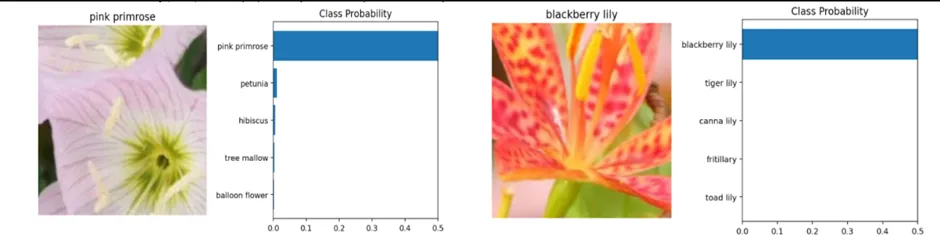
\includegraphics[width=1\textwidth]{imagenes/0005-fine-tuning.png}
                \caption{Fine-tuning en tareas de clasificación de flores usando el modelo pre-entrenado Restnet16 \cite{0005_journeyLLM,zhao2025surveylargelanguagemodels}}
                \label{fig:0005-fine-tuning}
            \end{figure}
            
            \noindent Los modelos pioneros como \textit{ELMo} \cite{zhao2025surveylargelanguagemodels} (Embeddings from Language Models) y \textit{BERT} \cite{zhao2025surveylargelanguagemodels} (Bidirectional Encoder Representations from Transformers) revolucionaron la forma en la que se procesaba el lenguaje natural (NLP) debido a la introducción de palabras representativas del contexto. Estos modelos agregaban al pre-entrenamiento, arquitecturas bidireccionales como \textit{Transformers}.
            
            \noindent Este pre-entrenamiento permitía a los modelos aprender las representaciones numéricas de palabras contextuales, gracias a los \textit{embeddings} (sección \ref{sec:embeddings}) y por consiguiente mejorar significativamente el rendimiento del NLP realizando pequeños ajustes (el llamado \textit{fine-tuning}). Modelos como \textit{GPT-2} \cite{zhao2025surveylargelanguagemodels} (Generative Pre-trained Transformer 2) y \textit{BART} \cite{zhao2025surveylargelanguagemodels} (Bidirectional and Auto-Regressive Transformers) surgieron en consecuencia y abrieron el camino a lo que hoy se conoce como los grandes modelos de lenguaje.

        \subsubsection{Grandes modelos de lenguaje (LLMs)}

            Los grandes modelos de lenguaje son el resultado de la ampliación progresiva de los PLMs. Este crecimiento en tamaño, acompañado del uso de conjuntos de entrenamiento cada vez más extensos y diversos, ha demostrado mejorar significativamente el rendimiento en múltiples tareas. Modelos recientes como \textit{GPT-4} han evidenciado comportamientos distintos respecto a sus predecesores más pequeños, mostrando una mayor capacidad para resolver tareas complejas sin necesidad de entrenamiento adicional.

            \noindent Actualmente, los LLMs están generando un impacto considerable en la comunidad de inteligencia artificial \cite{0005_journeyLLM}. Su desarrollo ha ampliado las expectativas sobre el potencial de estos modelos, hasta el punto de fomentar discusiones sobre una inteligencia artificial con capacidades que podrían igualar o incluso superar el razonamiento humano. Como ejemplo ilustrativo, el modelo \textit{GPT-4.5} ha sido recientemente citado por superar el test de Turing con un 73\% de éxito \cite{0006_ChatGPTuring}. Estas capacidades abren la puerta a aplicaciones que van desde el acceso avanzado al conocimiento y la automatización de tareas complejas, hasta la aceleración de descubrimientos científicos o el impulso económico.
            
            \noindent Una de las características más destacadas de los LLMs es la aparición de capacidades emergentes \cite{0005_journeyLLM}, es decir, habilidades que no estaban presentes en modelos más pequeños y que surgen como resultado del aumento de escala y del refinamiento en el entrenamiento.
            
            \subsubsection{Capacidades emergentes}
            
                El \textit{in-context learning} (aprendizaje en contexto) se refiere a la capacidad del modelo para resolver tareas a partir de ejemplos o instrucciones proporcionadas en la propia entrada del usuario (el prompt), sin necesidad de re-entrenar el modelo. Esta habilidad permite adaptar la respuesta al contexto ofrecido. Por ejemplo:
                
                \noindent \textit{Contexto: ``Eres un asistente virtual especializado en resolver problemas matemáticos."} \\
                \textit{Instrucción: ``Calcula la raíz cuadrada de 25."}
                
                \noindent De forma similar, el seguimiento de instrucciones es posible gracias a que muchos LLMs han sido ajustados utilizando conjuntos de datos formateados como instrucciones en lenguaje natural. Esto permite al modelo generalizar mejor a tareas nuevas, siempre que estén formuladas de manera instructiva.
                
                \noindent Por último, el razonamiento paso a paso hace referencia a la capacidad del modelo para descomponer un problema complejo en pasos más simples, facilitando así su resolución. Al encadenar instrucciones dentro de un \textit{prompt}, se puede guiar al modelo a pensar de forma más estructurada, lo que mejora tanto la precisión como la interpretabilidad de las respuestas generadas.

            \subsubsection{Aplicaciones de un LLM}

                En resumen, los grandes modelos de lenguaje tienen aplicaciones muy variadas que abarcan tanto direcciones de investigación como dominios específicos (ver figura \ref{fig:0006_llm_escena}). 
            
                \begin{figure}[H]
                    \centering
                    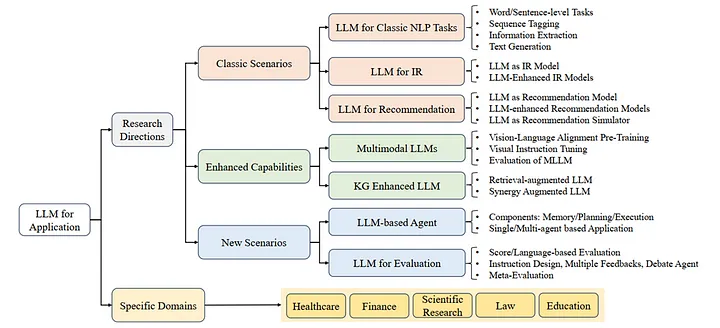
\includegraphics[width=1\textwidth]{imagenes/0006_llm_escena.png}
                    \caption{Esquema de las direcciones de investigación donde podemos usar LLMs \cite{0005_journeyLLM}, \cite{zhao2025surveylargelanguagemodels}}
                    \label{fig:0006_llm_escena}
                \end{figure}
                
                \noindent En el ámbito de las tareas clásicas del procesamiento del lenguaje natural, los LLMs son capaces de abordar actividades como el análisis a nivel de palabra u oración, el etiquetado de secuencias, la extracción de información y la generación de texto. En cuanto a la recuperación de información, estos modelos se utilizan como herramientas de búsqueda por sí mismas o para mejorar modelos existentes, incrementando la precisión y relevancia de los resultados obtenidos. También desempeñan un papel importante en los sistemas de recomendación, ya sea como modelos principales o como complemento de otros sistemas, simulando recomendaciones y ajustándose a las preferencias de los usuarios, como ocurre en plataformas como Netflix y YouTube \cite{0005_journeyLLM}.

                \noindent Los LLMs multi-modales representan otro avance importante, al ser capaces de integrar y procesar información proveniente de distintas modalidades, como texto e imágenes, mejorando así la interacción y comprensión de contenido en diferentes formatos. Asimismo, existen LLMs mejorados con grafos de conocimiento, los cuales incorporan datos estructurados para enriquecer su capacidad de comprensión y generación de contenido con un mayor contexto.
                
                \noindent Además de estas aplicaciones tradicionales, los LLMs se emplean en nuevos escenarios. Uno de ellos son los agentes basados en LLMs, que cuentan con capacidades de memoria, planificación y ejecución, permitiéndoles realizar tareas de manera autónoma y adaptarse a las solicitudes del usuario y al entorno. Otro caso es el uso de LLMs para evaluación, donde se aplican técnicas de evaluación para puntuar modelos o contenidos.
                
                \noindent En cuanto a dominios específicos, los LLMs han demostrado un rendimiento notable. En sanidad, modelos como Med-PaLM \cite{zhao2025surveylargelanguagemodels} han alcanzado un nivel experto en el Examen de Licencia Médica de EE.UU. , siendo aprobados por médicos en la resolución de preguntas médicas. En educación, herramientas como ChatGPT han ayudado a estudiantes a mejorar su rendimiento en asignaturas como seguridad informática, generando o refinando respuestas. En el ámbito legal, GPT-4 obtuvo una puntuación dentro del 10\% superior en un examen de acceso a la abogacía simulado, evidenciando su capacidad para la interpretación legal y el razonamiento. En finanzas, BloombergGPT \cite{zhao2025surveylargelanguagemodels} \cite{wu2023bloomberggptlargelanguagemodel} demostró un rendimiento destacado en múltiples tareas financieras, sin perder competitividad en tareas de propósito general. Por último, en la investigación científica, los LLMs han sido utilizados en distintas fases del proceso científico, incluyendo la revisión bibliográfica, la generación de hipótesis, el análisis de datos y la redacción de artículos. 

            \subsection{LLMs usados en el proyecto}
            \label{sec:cap2_llms_usados}

                Durante la realización del proyecto, hemos probado varios modelos de lenguaje, incluyendo modelos locales y externos. Los modelos seleccionados finalmente han sido tres, diferenciando las tres estrategias que podemos usar a la hora de usar un LLM, es decir: un modelo local, un modelo gratuito externo y un modelo externo de pago.

                \noindent En los siguientes apartados se explican con más detenimiento los modelos elegidos y las plataformas en los que están disponibles.

                \subsubsection{Llama 3.2}

                    Llama 3.2 \cite{0037_llama32} es modelo de lenguaje multilingüe perteneciente a Meta. Es una colección de modelos pre-entrenados diseñados para seguir instrucciones, con un tamaño de 1 a 3 billones de parámetros (1B y 3B). La versión usada en el proyecto es la 3B.

                    \noindent El modelo está optimizado para mantener conversaciones en varios idiomas, incluyendo tareas como la realización de agentes de búsqueda y resúmenes.
            
                    \begin{figure}[H]
                        \centering
                        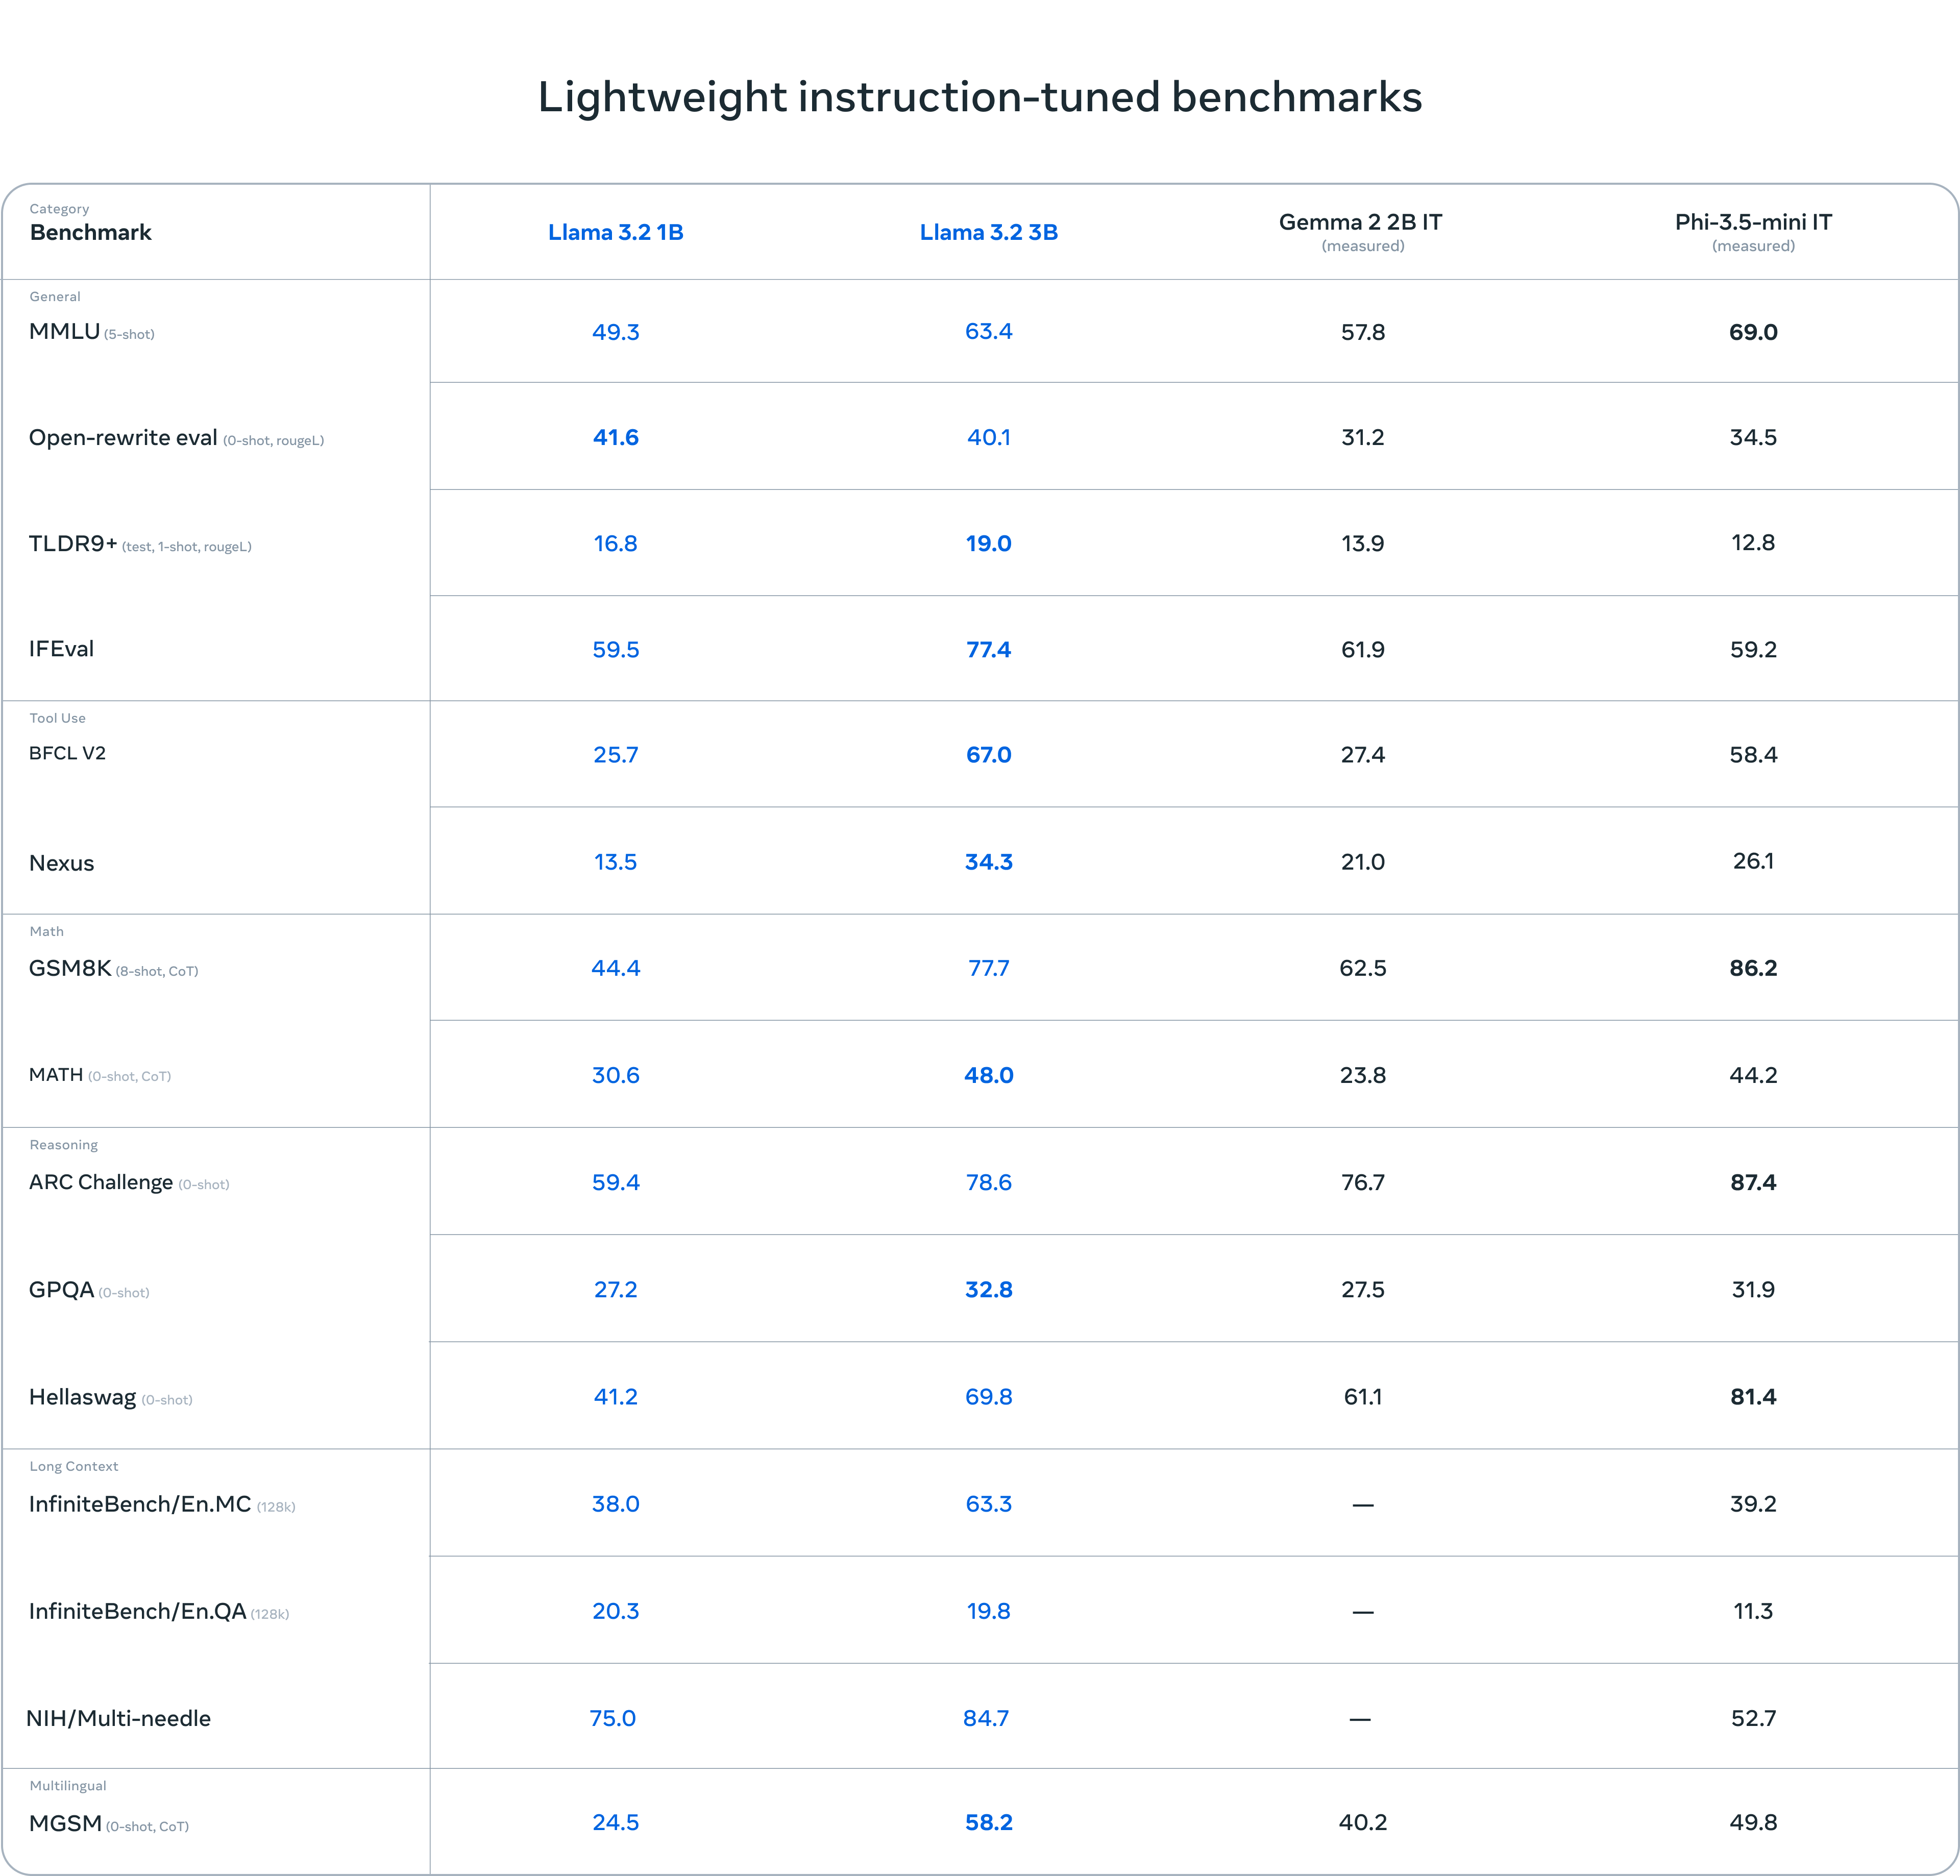
\includegraphics[width=1\textwidth]{imagenes/0090_llama32.png}
                        \caption{Tabla comparativa del modelo Llama 3.2 en diferentes benchmarks \cite{0037_llama32}}
                        \label{fig:0090_llama32}
                    \end{figure}

                    \noindent La plataforma donde esta disponible una versión de este modelo es Ollama (ver sección \ref{sec:ollama}). Es la opción que usaremos en el proyecto como base de pruebas de un modelo local, ya que la plataforma Ollama permite la descarga de multitud de modelo gratuitos.
                    
                \subsubsection{Mistral Small 3.2}

                    Mistral Small 3.2 \cite{0038_mistralsmall32} es la última actualización disponible del modelo Mistral Small. Este modelo mejora al anterior (Mistral Small 3.1 \cite{0039_mistralsmall31}) a la hora de dar respuestas precisas a instrucciones, generar menos texto repetitivo o generaciones infinitas.

                    \noindent El modelo Mistral Small 3.2 cuenta con un tamaño de 24 billones de parámetros (24B), algo considerable para ser usado localmente. Mistral AI ofrece este y otros modelos de forma gratuita a través de su API (con ciertas restricciones ratio/preguntas), por esa razón, es el modelo escogido para realizar las pruebas con un modelo externo gratuito.

                    \noindent \textbf{Nota:} La siguiente figura muestra el rendimiento del modelo 3.1. Mistral Small 3.2 es relativamente moderno (junio de 2025), y a día de hoy, no disponemos de un blog/página oficial que informe sobre su rendimiento actual.
            
                    \begin{figure}[H]
                        \centering
                        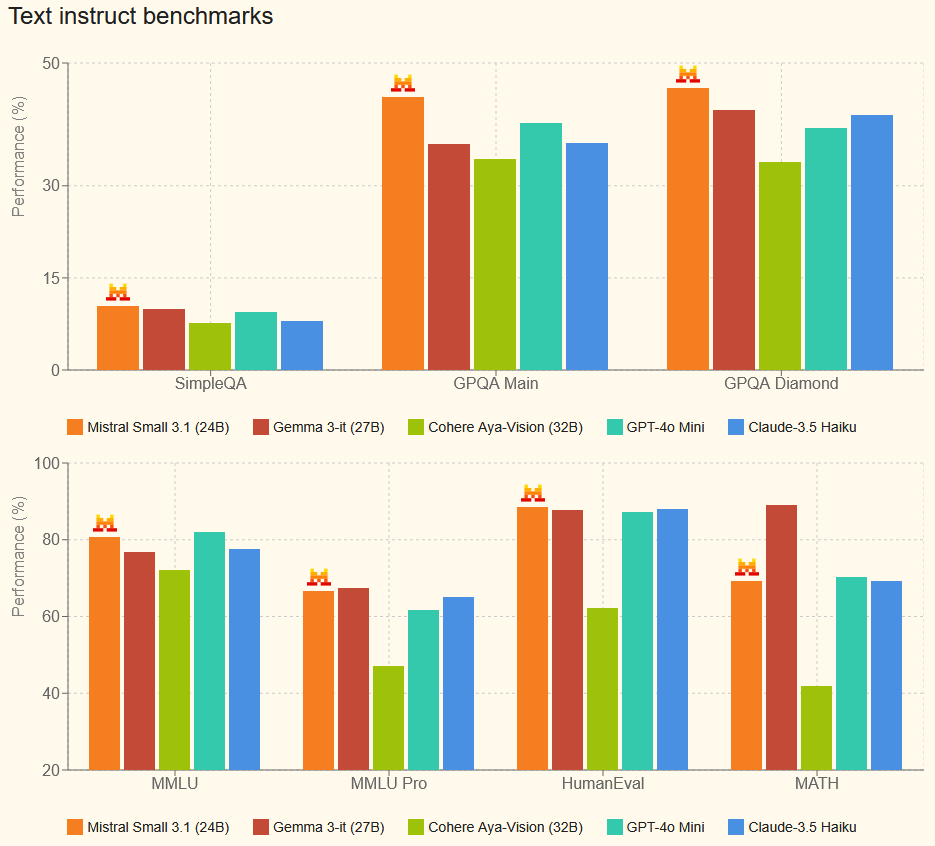
\includegraphics[width=.8\textwidth]{imagenes/0091_mistralsmall31.png}
                        \caption{Tabla comparativa del modelo Mistral Small 3.1 en diferentes benchmarks \cite{0039_mistralsmall31}}
                        \label{fig:0091_mistralsmall31}
                    \end{figure}

                \subsubsection{GPT-4.1}

                    El conjunto de modelos GPT-4.1 \cite{0043_gpt41} esta disponible en tres tamaños: GPT-4.1, GPT-4.1 Mini y GPT-4.1 Nano. Están destinados a programadores que necesitan un mayor rendimiento, un contexto más amplio y un seguimiento de las instrucciones más predecible. Cada modelo admite hasta 1 millón de tokens de contexto, un salto apreciable dado que los modelos anteriores permitían un tamaño de contexto de 128 mil.
                    
                    \noindent GPT-4.1 mejora las capacidades de GPT-4o, manteniendo la latencia más o menos en el mismo rango. En la práctica, significa que podemos obtener mejor rendimiento sin pagar un coste en capacidad de respuesta (ver figura \ref{fig:0121_gptprecios} para ver los precios). En la siguiente figura, GPT-4.1 adelanta en inteligencia a GPT-4o manteniendo una velocidad similar. De igual manera, la versión \textit{mini} es más inteligente siendo un poco más lenta.
                    
                    \begin{figure}[H]
                    	\centering
                    	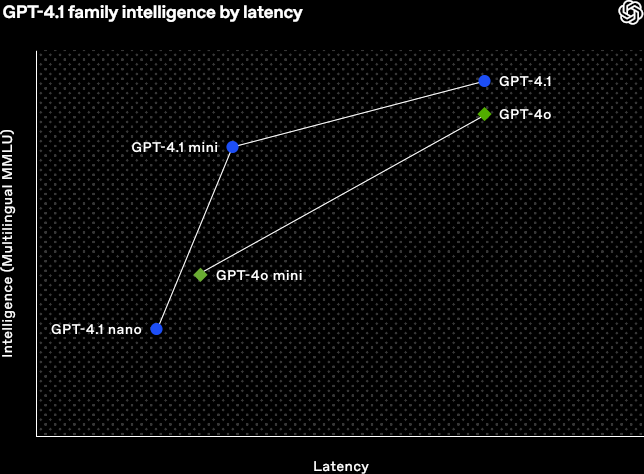
\includegraphics[width=.8\textwidth]{imagenes/0120_gpt41.png}
                    	\caption{Rendimiento del conjunto de modelos GPT-4.1 \cite{0043_gpt41_2}}
                    	\label{fig:0120_gpt41}
                    \end{figure}
                    
                    \begin{figure}[H]
                    	\centering
                    	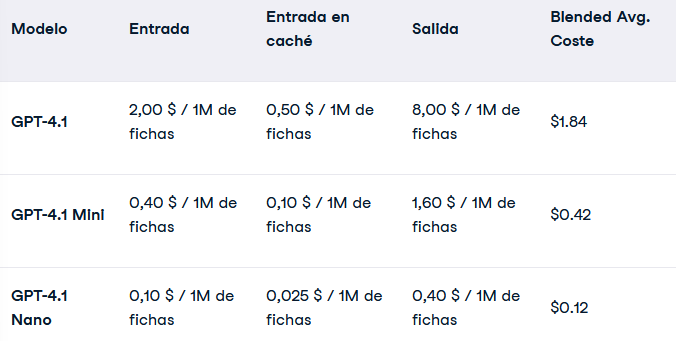
\includegraphics[width=.8\textwidth]{imagenes/0121_gptprecios.png}
                    	\caption{Precio de los modelos GPT-4.1 \cite{0043_gpt41_2}}
                    	\label{fig:0121_gptprecios}
                    \end{figure}
                    
                    \noindent El modelo GPT-4.1 es el escogido realizar las pruebas, para lo cual necesitaremos conseguir una de las claves API disponibles en la plataforma de OpenAI. Siempre que tengamos créditos en la cuenta podemos acceder al modelo, por lo que hay que tener en cuenta este factor. Con este modelo de pago, ya tenemos todos los modelos de los que queremos evaluar su rendimiento en nuestro proyecto.


    \section{Modelos de Embedding}
    \label{sec:embeddings}

        Los modelos de embedding son la parte esencial en el modelo de recuperación de información de un sistema RAG, ya que permiten transformar datos complejos como texto, imágenes o audio \cite{0007_Embeddings}; en representaciones vectoriales densas y de baja dimensión. Estas representaciones conservan relaciones semánticas relevantes y resultan mucho más manejables para recuperar documentos relevantes dada una consulta de usuario.
    
        \begin{figure}[H]
            \centering
            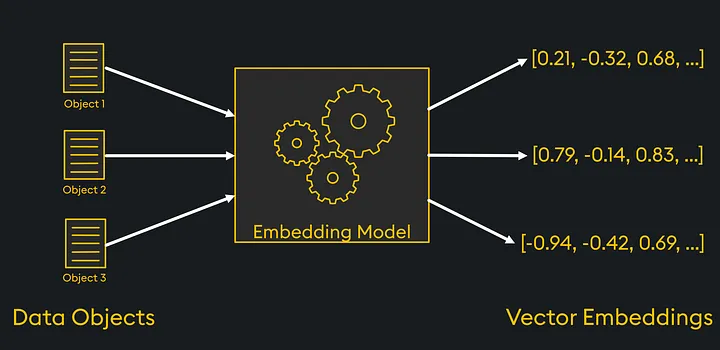
\includegraphics[width=0.7\textwidth]{imagenes/0007-ej-embeddings.png}
            \caption{Ejemplo básico de funcionamiento de un modelo de embeddings \cite{0007_Embeddings}. Recibe objetos de datos, que pueden ser de todo tipo, y los transforma en una representación vectorial}
            \label{fig:0007-ej-embeddings}
        \end{figure}
            
        \noindent Por otra parte, los embeddings también son una pieza fundamental en multitud de técnicas de aprendizaje automático. Los vectores generados pueden emplearse en tareas como clasificación, agrupamiento (clustering), recomendación o recuperación de información, etc. 
        
        \noindent Gracias a su versatilidad, los modelos de embedding se utilizan en una amplia variedad de aplicaciones del mundo real. En sistemas de análisis de sentimientos, permiten identificar matices emocionales en el texto a partir de la representación semántica de las palabras. En sistemas de recomendación, se emplean para medir similitudes entre usuarios y productos, ofreciendo sugerencias personalizadas. En tareas de respuesta automática a preguntas, los embeddings permiten emparejar preguntas y respuestas en función de su similitud semántica, facilitando la recuperación de la respuesta más adecuada. Finalmente, debido a que estos modelos pueden representar palabras y frases en múltiples idiomas dentro de un mismo espacio vectorial, también resultan especialmente útiles en tareas de traducción automática, donde es posible identificar significados equivalentes entre lenguas diferentes \cite{0007_Embeddings}.
            
        \noindent En resumen, los modelos embeddings son una herramienta clave para representar datos de forma compacta y significativa, lo que habilita una gran variedad de aplicaciones en el campo del aprendizaje automático y el procesamiento del lenguaje natural.

        \noindent En las siguientes sub-secciones hablaremos de los modelos de embeddings utilizados en nuestro sistema RAG.

        \subsection{Nomic Embed (nomic-embed-text)}

            \textbf{Nomic Embed} \cite{0024_nomic} es un modelo avanzado de embedding de texto desarrollado por \textbf{Nomic}, diseñado para ofrecer una capacidad excepcional en tareas tanto de corto como de largo contexto. Este modelo sobresale frente a alternativas como \textit{Ada-002} o \textit{text-embedding-3-small} de OpenAI (figura \ref{fig:0048_nomic}), gracias a su enfoque en la accesibilidad y auditabilidad completa del modelo.
    
            \begin{figure}[H]
                \centering
                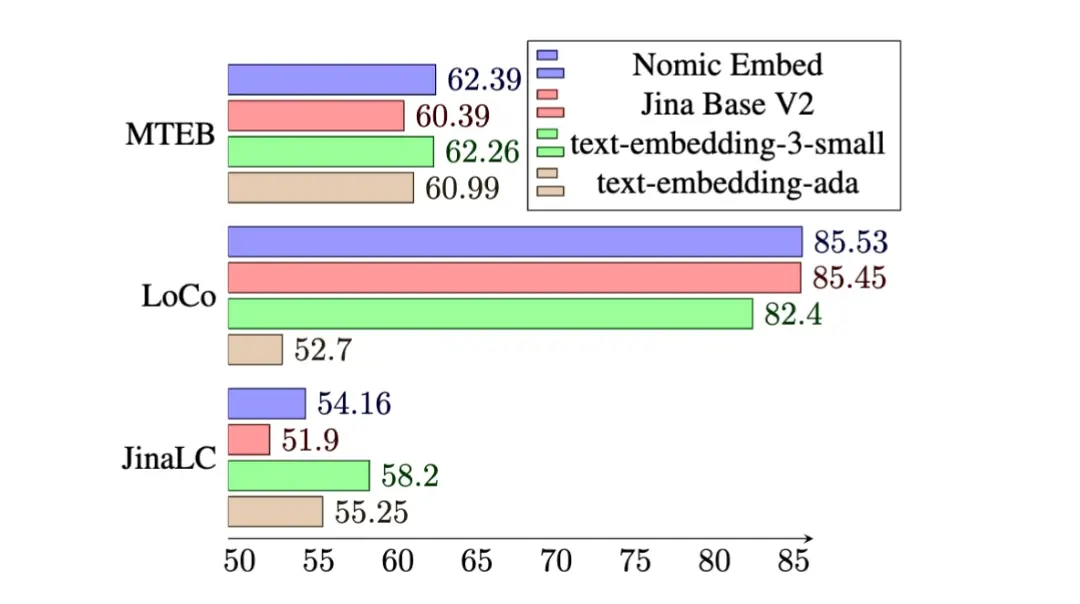
\includegraphics[width=0.8\textwidth]{imagenes/0048_nomic.png}
                \caption{Rendimiento comparativo de Nomic Embed y otros modelos en distintos benchmarks \cite{0024_nomic}}
                \label{fig:0048_nomic}
            \end{figure}

            \noindent Las características destacadas de este modelo \cite{0024_nomic} se pueden resumir en: código abierto y rendimiento. Nomic Embed se distingue por su enfoque abierto completamente abierto, incluyendo datos de entrenamiento, código de entrenamiento y modelos bajo licencia Apache2.

            \noindent Evaluado en benchmarks como \textit{MTEB} y \textit{LoCo} (figura \ref{fig:0048_nomic}), Nomic Embed supera a modelos líderes en tareas de largo contexto, demostrando consistencia y superioridad en entornos supervisados y no supervisados.       

            \noindent En resumen, nomic Embed se posiciona como una opción muy recomendable para proyectos que buscan integrar modelos de embedding de texto avanzados y completamente auditables.

        \subsection{BGE-M3}        

            BGE-M3 \cite{0025_bge-m3} es otro modelo de embedding de texto basado en la arquitectura \textit{XLM-RoBERTa}, diseñado para ser altamente versátil en diversos escenarios de recuperación de información. Su nombre proviene de sus tres capacidades:

            \begin{itemize}
                \item \textbf{Multi-funcionalidad}: BGE-M3 es capaz de realizar de manera simultánea recuperación densa, recuperación con multiples vectores y recuperación dispersa, ampliando significateivamente su rango de aplicación.
                \item \textbf{Multilingüe}: Este modelo ofrece soporte para más de cien idiomas, lo que lo convierte en una herramienta eficaz en contextos multilingües y de alcance global.
                \item \textbf{Multi-granularidad}: Puede procesar texto con distintos niveles de granularidad, desde frases cortas hasta documentos de hasta 8192 tokens de longitud.
            \end{itemize}
    
            \begin{figure}[H]
                \centering
                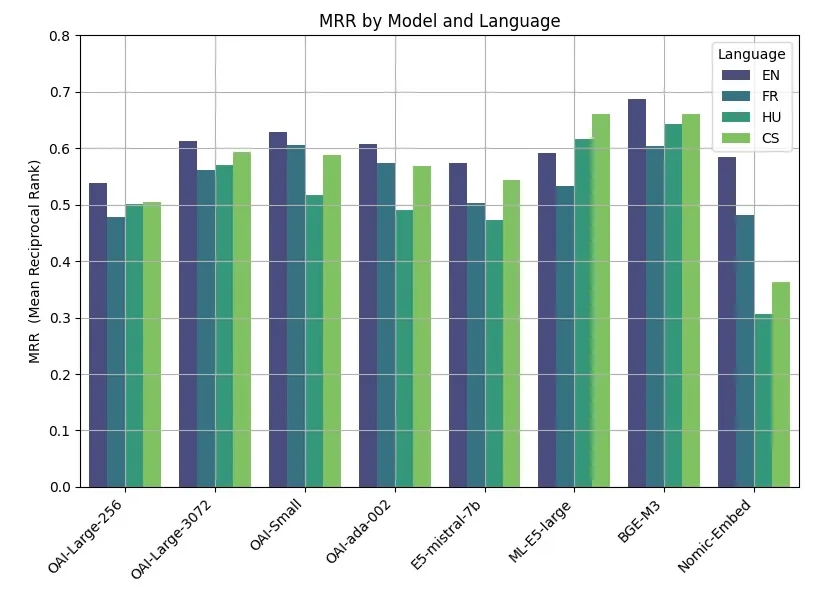
\includegraphics[width=0.8\textwidth]{imagenes/0049_bge-m3.png}
                \caption{Rendimiento comparativo del modelo bge-m3 con otros modelos \cite{0025_bge-m3}}
                \label{fig:0049_bge-m3}
            \end{figure}

            \noindent Definitivamente, BGE-M3 resulta ideal para sistemas de búsqueda semántica multilingüe y cualquier entorno donde se requiera una compresión profunda del texto en múltiples idiomas. Su enfoque multifuncional representa un avance significativo en el desarrollo de modelos de embedding flexibles, escalables y multilingües.

        \subsection{Artic Embed 2.0 (snowflake-arctic-embed2}

            El modelo Artic Embed 2.0 \cite{0026_snowflake}, desarrollado por Snowflake, representa la nueva iteración en sus modelos de embedding \textit{frontier}. Esta nueva versión incorpora soporte multilingüe sin comprometer su rendimiento o escalabilidad.
    
            \begin{figure}[H]
                \centering
                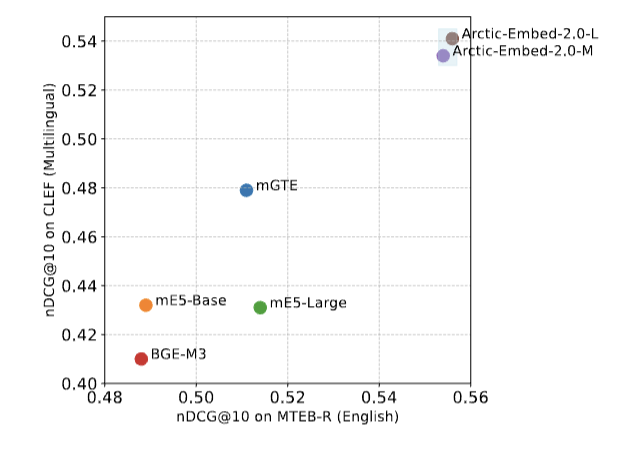
\includegraphics[width=0.8\textwidth]{imagenes/0050_snowflake.png}
                \caption{Métricas obtenidas por los modelos de Artic Embed en comparación con otros, usando el benchmark MTEB-R en inglés. \cite{0026_snowflake}}
                \label{fig:0050_snowflake}
            \end{figure}

            \noindent Artic Embed 2.0 logra resultados altos en tareas de recuperación semántica tanto en inglés como en otros idiomas europeos, demostrando una notable capacidad de generalización incluso en lenguas no vistas durante el entrenamiento.

            \noindent Snowflake ha diseñado este modelo pensando el entornos de alta demanda, ofreciendo latencias de 10ms por consulta. Incluye una compresión eficiente (MRL, Matryoshka Representation Learning) que permite búsquedas rápidas y económicas en grandes conjuntos de datos.
            
            \noindent Este modelo se distribuye bajo una licencia de uso Apache 2.0, permitiendo su libre uso.

            \noindent En resumen, Snowflake ofrece un modelo de embedding con soporte multilenguaje, capacidad de compresión y orientado a entornos empresariales.

        \subsection{Jina Embeddings v2 Base ES ( jina-embeddings-v2-base-es)}

            El modelo de embedding bilingüe español-inglés \textit{jina-embeddings-v2-base-es} \cite{0027_jina}, desarrollado por Jina AI, está diseñado para aplicaciones que requieren representaciones semánticas robustas en cualquiera de estos dos idiomas. 

            \noindent Basado en una arquitectura BERT (JinaBERT), este modelo esta pensado para ofrecer un alto rendimiento en aplicaciones monolingües y bilingües ya que ha sido entrenado específicamente para admitir entradas de español e inglés sin sesgo.

            \noindent Además, su tamaño se ubica entre los más ligeros entre los embeddings multilingües disponibles, facilitando su implementación en entornos con recursos limitados.

            \noindent Por último, puede integrarse fácilmente vía Python a través de Ollama, y es apto para sistemas RAG según pruebas recientes con LlamaIndex (ver figura \ref{fig:0051_jina}).             
    
            \begin{figure}[H]
                \centering
                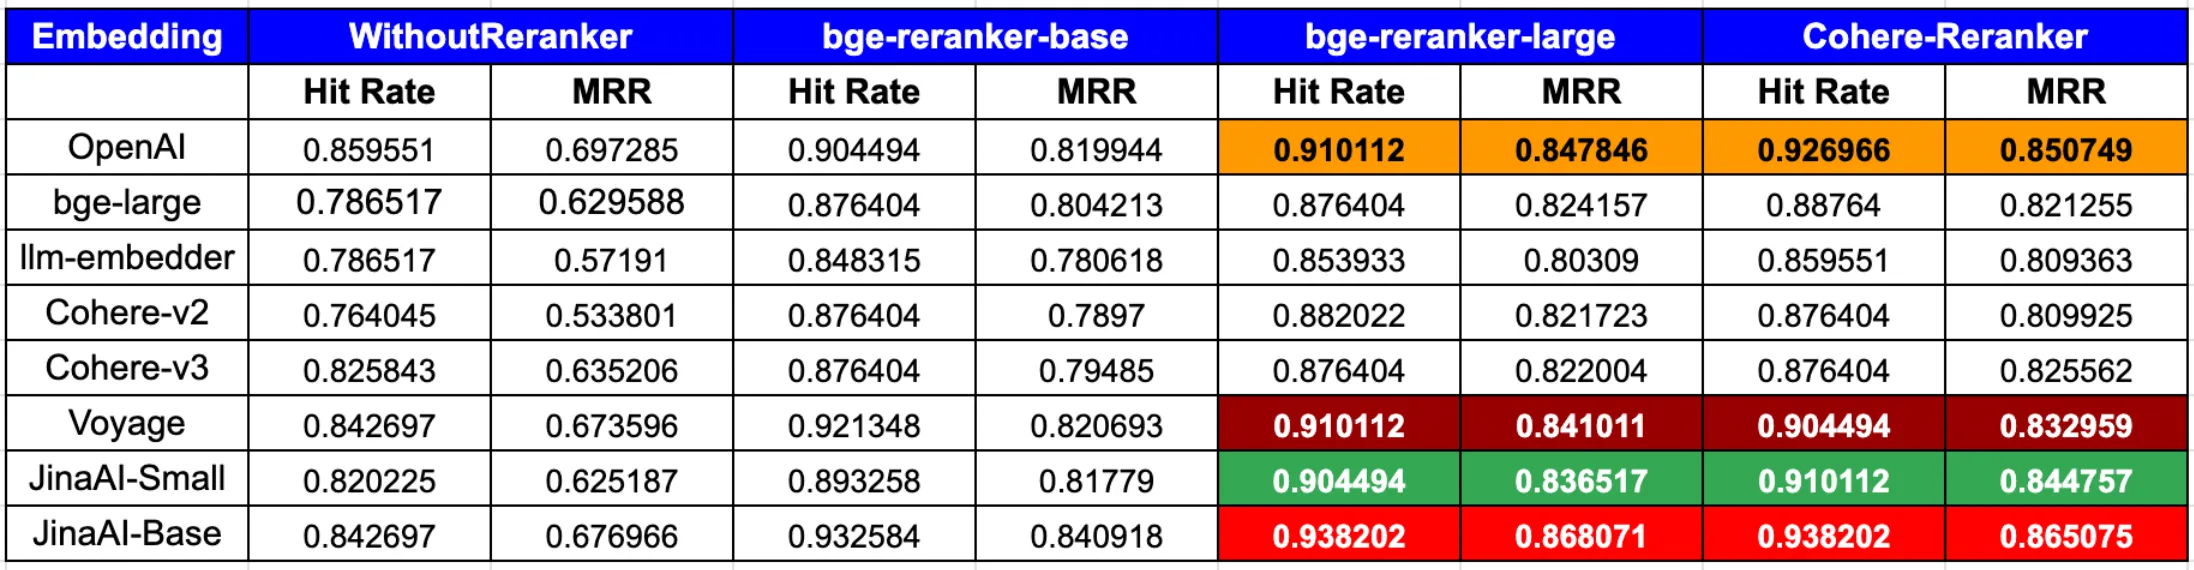
\includegraphics[width=1\textwidth]{imagenes/0051_jina.png}
                \caption{Comparación de varios modelos de embedding con JINA. \cite{0027_jina}}
                \label{fig:0051_jina}
            \end{figure}

        \subsection{Text Embedding 3 (text-embedding-3-small)}

            El modelo \textit{text-embedding-3-small} es una versión mejorada y eficiente del modelo de embedding anterior \textit{text-embedding-ada-002}, ambos pertenecientes a \textbf{OpenAI} \cite{0040_openai_embed}.                  

            \noindent Como se puede observar en la figura \ref{fig:0097_te3s}, la puntuación media en una prueba comparativa de uso común para la recuperación en varias lenguas (MIRACL) aumento de un 31,4\% hasta el 44\%, mientras que la puntuación media para tareas en inglés (MTEB) aumento del 61\% hasta el 62,3\%.
    
            \begin{figure}[H]
                \centering
                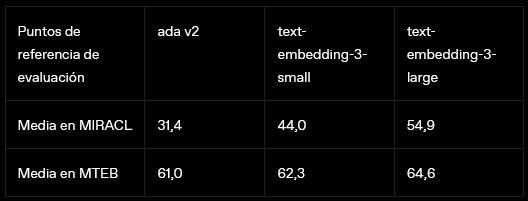
\includegraphics[width=.7\textwidth]{imagenes/0097_te3s.png}
                \caption{Evaluaciones de los modelos de embedding de OpenAI \cite{0040_openai_embed}}
                \label{fig:0097_te3s}
            \end{figure}

            \noindent El precio de uso también se ha reducido al ser un modelo más eficiente que el anterior, casi cinco veces.

            \noindent Este modelo ha sido entrenado con una técnica que permite a los desarrolladores equilibrar el rendimiento y costes al utilizar las integraciones, podemos acortarlas sin perder sus propiedades de representación de conceptos (ver figura \ref{fig:0098_te3s_2}).
            
            \begin{figure}[H]
            	\centering
            	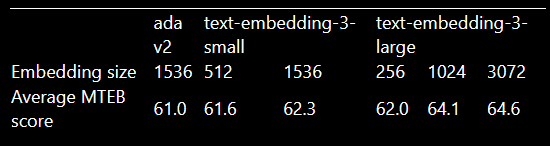
\includegraphics[width=.7\textwidth]{imagenes/0098_te3s_2.png}
            	\caption{Evaluaciones de los modelos de embedding de OpenAI con distintos tamaños \cite{0040_openai_embed}}
            	\label{fig:0098_te3s_2}
            \end{figure} 
            
            \noindent De este modo se logra un uso altamente flexible, permitiendo utilizar almacenes de datos vectoriales más optimizados sin perder rendimiento.

    \section{Alternativa al uso de LLM: RASA Pro}

        En esta sección abordaremos una alternativa al uso de los LLMs, \textbf{Rasa Pro}. En un principio este proyecto iba a ser desarrollado usando la herramienta Rasa Open Source, un framework gratuito de RASA para la creación de asistentes conversacionales basado en el entrenamiento de una red neuronal con un conjunto de ``intenciones" de usuario y de respuestas asociadas.

        \noindent Rasa se consolidó como una de las principales plataformas para el desarrollo de asistentes conversacionales gracias a que ofrecían un marco flexible basado en el procesamiento del lenguaje natural y el aprendizaje automático. Sin embargo, los modelos tradicionales usados por Rasa, limitan su capacidad para comprender consultas complejas o para responder de una forma natural, a parte de la necesaria actualización de la red para cada cambio realizado.

        \noindent En ese contexto surgió Rasa Pro, la versión empresarial de Rasa. Rasa Pro incorpora funcionalidades avanzadas que aprovechan las capacidades de los LLMs. Uno de los aspectos clave es el uso de CALM (Conversational AI for Language Models \cite{0008_RasaCalm}), un enfoque que combina la flexibilidad de Rasa para gestionar diálogos con la potencia de un modelo de lenguaje. Esta integración permite obtener respuestas más naturales y contextualizadas, mejorar de entradas de usuario ambiguas y reducir el tiempo de entrenamiento.

        \noindent A continuación, apreciaremos algunas de las características diferenciadoras con Rasa Open Source, y también, expondremos el porque hemos optado por el uso de LLMs tradicionales en vez de esta herramienta.

        \subsection{Licencia de uso}

            Rasa Pro es un producto que requiere de una licencia de uso, siendo esta uno de sus principales inconvenientes. Aunque es posible obtener una licencia para desarrolladores de manera gratuita, esta presenta ciertas limitaciones:

            \begin{itemize}
                \item Límite de 1000 conversaciones mensuales, 100 para asistentes internos dirigidos a empleados.
                \item Uso restringido a un sólo usuario.
                \item Permite su uso en entornos comerciales, pero tiene restricciones especificadas en la licencia.
                \item Validez de cada clave de 12 meses.
            \end{itemize}

            \noindent Encontramos dos problemas clave en la lista anterior. En primer lugar, aunque la licencia es gratuita requiere de una renovación anual, lo que puede presentar un problema a largo plazo. El segundo inconveniente, es un límite de conversaciones mensuales demasiado bajo para las necesidades de cualquier proyecto medianamente ``importante", y que presenta una desventaja muy grande en comparación con otras soluciones de código abierto, las cuales no imponen restricciones de uso y son completamente gratuitas. 

        \subsection{Facilidad de uso}

            Un primer vistazo a la estructura y al código generado por Rasa Pro, nos permite observar que, aunque se ha mantenido la misma estructura de proyecto, se han sustituido los ficheros de la carpeta \textit{data} por otros nuevos (ver figura \ref{fig:0008-comparacionEstructuras}).

            \begin{figure}[H]
                \centering
                \begin{subfigure}{0.45\textwidth}
                    \centering
					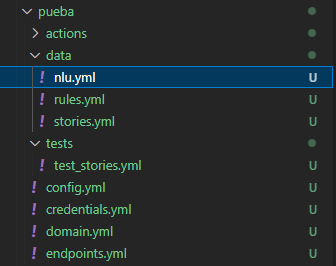
\includegraphics[width=0.8\textwidth]{imagenes/0008a-estructuraRasa.png}
					\caption{Estructura de Rasa}
                \end{subfigure}   
                \begin{subfigure}{0.45\textwidth}
                    \centering
					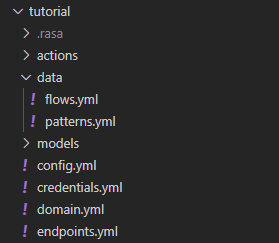
\includegraphics[width=0.8\textwidth]{imagenes/0008b-estructuraRasaPro.png}
					\caption{Estructura de Rasa Pro}
                \end{subfigure}                  
				\caption{Comparación de las dos estructuras}
				\label{fig:0008-comparacionEstructuras}
            \end{figure}

            \noindent Estos nuevos archivos engloban los flujos de conversación (ver figura \ref{fig:0009-ficheroNuevos}) que el asistente debe seguir. Los flujos están diseñados para recoger toda la información necesaria para realizar el proceso que tienen programado.

            \begin{figure}[H]
                \centering
                \begin{subfigure}{0.49\textwidth}
                    \centering
					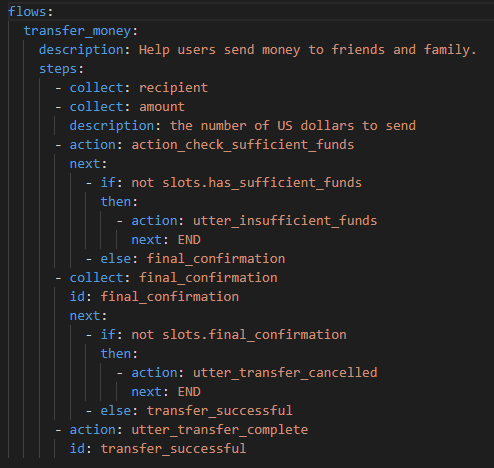
\includegraphics[width=0.9\textwidth]{imagenes/0009a-flows.png}
					\caption{flows.yml}
                \end{subfigure}   
                \begin{subfigure}{0.45\textwidth}
                    \centering
					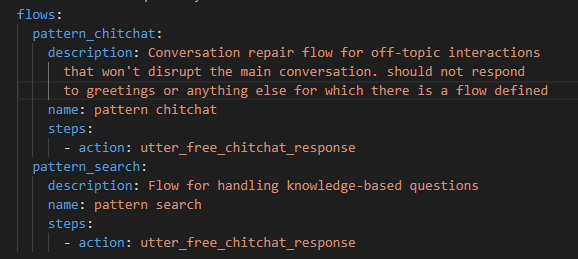
\includegraphics[width=0.9\textwidth]{imagenes/0009b-patterns.png}
					\caption{patterns.yml}
                \end{subfigure}                  
				\caption{Contenido de los ficheros flows.yml y patterns.yml}
				\label{fig:0009-ficheroNuevos}
            \end{figure}

            \noindent Los llamados \textit{Slots} (la memoria del asistente) son leídos en el flujo mediante la etiqueta \textit{collect} y son manejados, al igual que las respuestas, de la misma manera que con Rasa Open Source, en el archivo \textit{domain.yml}. Es posible añadir un prompt en este archivo para ayudar al modelo a manejar las respuestas (ver figura \ref{fig:0010-respuestaPrompt})

            \begin{figure}[H]
                \centering
                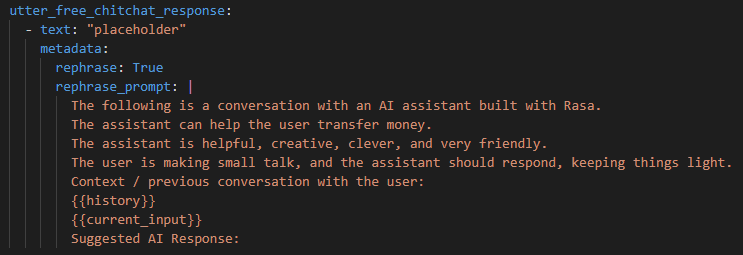
\includegraphics[width=0.9\textwidth]{imagenes/0010-respuestaPrompt.png}
                \caption{Ejemplo de una respuesta con prompt integrado}
                \label{fig:0010-respuestaPrompt}
            \end{figure}

            \noindent En resumen, los cambios que aporta esta versión hacen que controlar el flujo de conversación sea más sencillo y claro. Ahora las intenciones de usuario, son deducidas gracias al uso de modelos de lenguaje. El código es fácil de adaptar a las necesidades de cualquier proyecto y permite controlar las respuestas dadas por el asistente, debido a que todo este permanece \textit{on premise}.

        \subsection{Rendimiento}

            El asistente de prueba de Rasa Pro usa por defecto un modelo de lenguaje desarrollado por la misma empresa: \textbf{codellama} \cite{0009_CodeLlama}. Este modelo ya esta preparado para usarse en asistentes implementados bajo el CALM, es decir, este modelo traduce los mensajes enviados por un usuario a los comandos que son necesarios para avanzar en la conversación. De acuerdo a la documentación, este modelo no es capaz de generar texto arbitrario o creativas, ni texto problemático o dañino.

            \noindent A la hora de probar el modelo, Rasa Pro incluye un modo ``inspector", nos permite visualizar en una interfaz de navegador un grafo con el flujo de conversación en tiempo real (ver figura \ref{fig:0011-grafoFlujo}).      

            \begin{figure}[H]
                \centering
                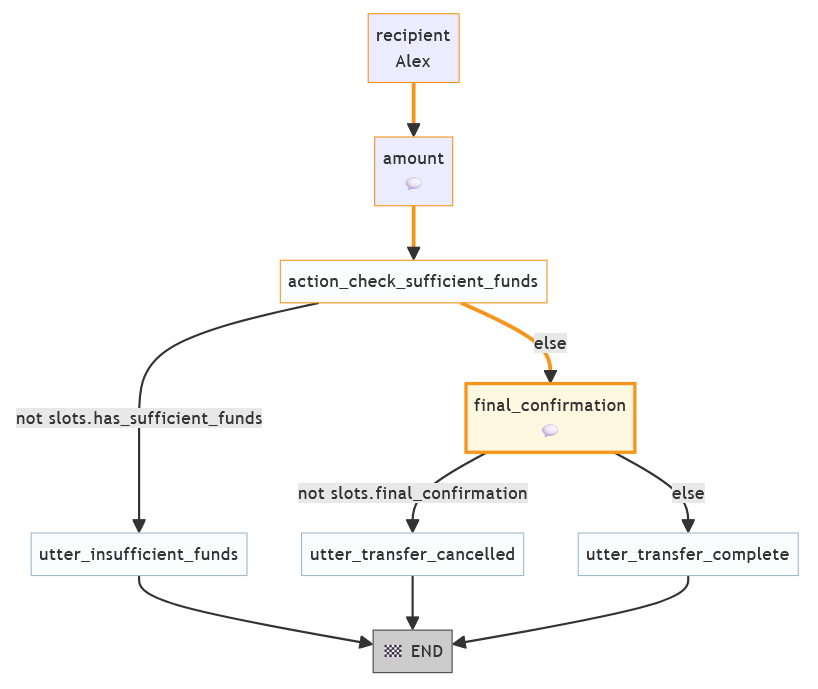
\includegraphics[width=.8\textwidth]{imagenes/0011-grafoFlujo.png}
                \caption{El inspector nos muestra un grafo con el flujo de conversación}
                \label{fig:0011-grafoFlujo}
            \end{figure}

            \noindent Otro aspecto importante es, que en las conversaciones podemos optar por dar los datos uno a uno o todos a la vez (ver figura \ref{fig:0012-convers}). Esta característica ya estaba presente en la versión anterior de Rasa (Rasa Open Source) y en esta la han mantenido.

            \begin{figure}[H]
                \centering
                \begin{subfigure}{0.49\textwidth}
                    \centering
					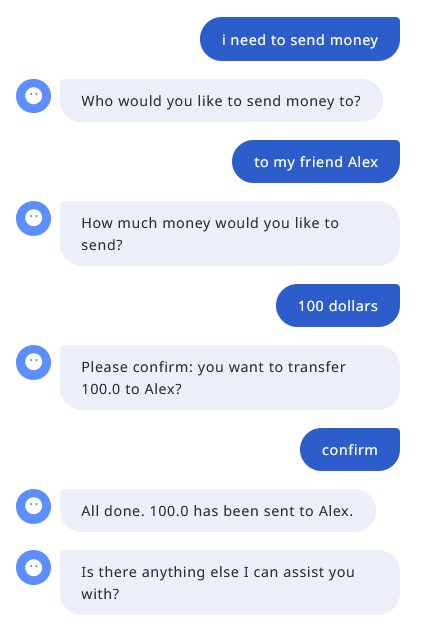
\includegraphics[width=0.9\textwidth]{imagenes/0012a-conversacion1.png}
					\caption{Datos uno a uno}
                \end{subfigure}   
                \begin{subfigure}{0.45\textwidth}
                    \centering
					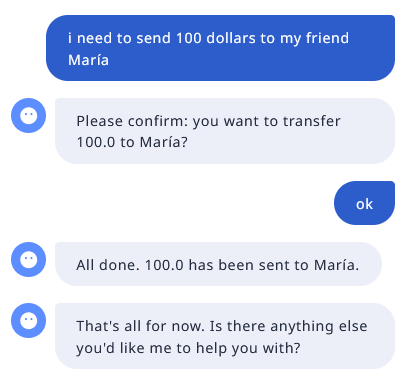
\includegraphics[width=0.9\textwidth]{imagenes/0012b-conversación.png}
					\caption{Todos los datos a la vez}
                \end{subfigure}                  
				\caption{Maneras en las que puedes conversar en una aplicación hecha con Rasa Pro}
				\label{fig:0012-convers}
            \end{figure}

            \noindent En cuanto al rendimiento, el tiempo de ejecución del modelo de prueba es casi inmediato. Sin embargo, como hemos mencionado anteriormente, la imposibilidad de este modelo a generar respuestas creativas, lo convierten en una opción no muy recomendable. 

            \noindent Rasa Pro permite modificar el modelo de lenguaje dentro de la configuración del proyecto, ofreciendo compatibilidad con modelos tanto locales como en la nube, incluyendo OpenAI y otras alternativas.

            \noindent En nuestras pruebas, utilizamos un modelo local \textit{llama3.2} descargado gracias a la plataforma \textbf{Ollama } (ver sección \ref{sec:ollama}). Los resultados obtenidos no fueron muy buenos, además de presentar tiempos de respuesta significativamente altos en comparación con el modelo anterior, en ocasiones omitía pasos dentro de la conversación. No se realizaron pruebas con modelos de OpenAI debido a la falta de clave de acceso a sus servicios.

            \subsection{Conclusión respecto a Rasa Pro}

                La integración de base de Rasa Pro con los modelos de lenguaje representa un avance significativo para el desarrollo de asistentes conversacionales en esta plataforma. Con la adopción del enfoque CALM \cite{0008_RasaCalm}, podemos gestionar diálogos de una forma más dinámica eliminando la necesidad de definir las intenciones explícitamente.

                \noindent Sin embargo y, como hemos mencionado en anteriores apartados, Rasa Pro cuenta con una serie de limitaciones que deben ser consideradas. Las restricciones puestas por su licencia gratuita pueden ser un obstáculo para aplicaciones que requieran una más alta cantidad de interacciones. El modelo de lenguaje de prueba incorporado, aunque ofrece respuestas en muy poco tiempo, su capacidad de generar respuestas es también limitada y puede no ajustarse a todos los casos de uso.

                \noindent En nuestras pruebas, el uso de modelos de lenguajes locales no logró resultados satisfactorios debido a unos tiempos de respuesta muy elevados y ciertas inconsistencias en la generación de respuestas.

                \noindent En definitiva, aunque Rasa Pro es una opción potente y viable para desarrollar asistentes conversacionales, presenta bastantes inconvenientes. Las limitaciones que tenemos tanto por la licencia como por el uso de modelos de lenguaje locales, nos hacen movernos hacia otras opciones de código libre (algunas ya mencionadas), que no requieren de licencia o que no ponen restricciones de uso.
    
    \section{Ollama}
    \label{sec:ollama}
        
        Ollama \cite{0010_Ollama1} es una herramienta de código abierto en la que podemos usar LLMs disponibles gratuitamente en nuestra propia máquina local (o servidor). Ollama actúa como un puente entre el modelo de lenguaje y nuestra máquina, no solo permitiéndonos usarlo, si no que también ofreciendo una API que podemos usar en aplicaciones más avanzadas.        

        \begin{figure}[H]
            \centering
            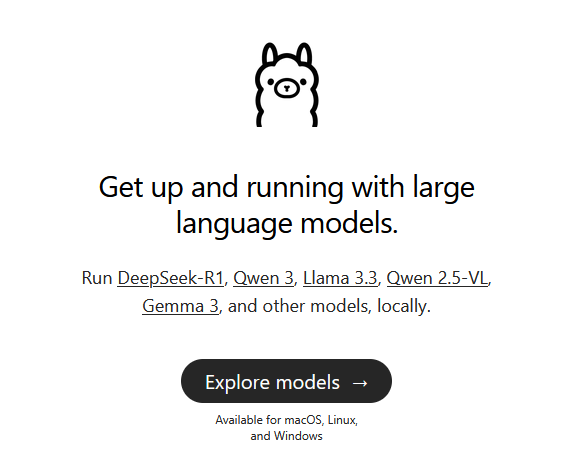
\includegraphics[width=.8\textwidth]{imagenes/0013_ollama.png}
            \caption{Sitio web oficial de Ollama: \url{https://ollama.com/}}
            \label{fig:0013_ollama}
        \end{figure}

        \noindent Al acceder localmente a los modelos, podemos mantener un control total sobre los datos y, evitar la inseguridad o los riesgos asociados con los servicios en la nube. Además, las herramientas sin conexión que ofrece Ollama ayudan a reducir latencias y dependencias de servidores externos, haciéndolas más rápidas (dependiendo mucho del equipo en el se ejecute) y confiables.

        \noindent En los siguientes apartados, repasaremos algunas de las características más importantes de esta herramienta y mostraremos un ejemplo de uso.
        
        \subsection{Características principales de Ollama}

            \subsubsection{Privacidad y acceso sin conexión}

                Es una de las principales características \cite{0010_Ollama1} que ofrece Ollama, la cual nos da la opción de ejecutar modelos de forma privada en nuestra máquina y sin conexión a Internet. De esta manera, podemos mantener nuestros datos de forma privada en nuestra equipo local sin que sean enviados a través de la red. Esta es una gran ventaja de Ollama sobre otros servicios en la nube, que podrían usar nuestros datos para otros propósitos.

            \subsubsection{Manejo de modelos}

                Añadir modelos a nuestra librería \cite{0010_Ollama1} local de Ollama es un proceso muy sencillo (tal y como se describe en la sección \ref{sec:ints&func_Ollama}). En el momento de escribir esta memoria el repositorio de Ollama cuenta con más de 150 modelos listos para usarse, desde \textit{Deepseek R1} hasta otros más populares como \textit{Llama3}, \textit{Gemma3}, \textit{Qwen2.5} o \textit{Mistral}. La web oficial de Ollama cuenta con la lista de los modelos disponibles.

            \subsubsection{Integración sencilla}

                Ollama se puede integrar fácilmente con una amplia variedad de herramientas, librerías y lenguajes de programación, por lo que es sencillo para los programadores incorporar LLMs en su flujo de trabajo \cite{0010_Ollama1,0011_Ollama2}. A parte de \textit{Python}, \textit{LangChain} (ver sección \ref{sec:LangChain}) o \textit{LlamaIndex}, Ollama presenta unas opciones de integración efectivas para el desarrollo de aplicaciones y soluciones avanzadas basadas en la IA.

            \subsubsection{Personalización y ajuste (Fine-tuning)}

                Ollama también nos da la posibilidad de ajustar ciertos parámetros de los modelos, como por ejemplo el tamaño de la ventana de contexto que usa el modelo para generar su respuesta o la temperatura/creatividad al generar la misma. Además, Ollama incluye el mecanismo \textit{modelfile}, en el cual podemos editar los parámetros del modelo usando un modelo base (un ejemplo es mostrado en la figura \ref{fig:0014_ollama_modelfile}).

                \begin{figure}[H]
                    \centering
                    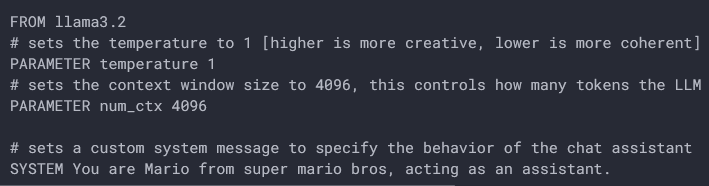
\includegraphics[width=.8\textwidth]{imagenes/0014_ollama_modelfile.png}
                    \caption{Fichero \textit{modelfile} básico, edita la temperatura y la ventana del contexto del modelo. Tiene de base el LLM \textit{Llama3.2}}
                    \label{fig:0014_ollama_modelfile}
                \end{figure}
                
        \subsection{Instalación y funcionamiento de Ollama}
        \label{sec:ints&func_Ollama}

            El archivo de instalación de Ollama se encuentra en su página web oficial, hay disponibles tres versiones para su descarga: \textit{Linux}, \textit{macOS} y \textit{Windows}. La instalación en \textit{Windows} no difiere de cualquier otro software para este sistema operativo, las otras dos versiones requieren de usar la consola para la instalación:

            \begin{itemize}            
                \item Para \textit{Linux}:
                    \begin{verbatim}
                        chmod +x ollama_linux.sh 
                        ./ollama_linux.sh
                    \end{verbatim}
                \item Para \textit{macOS}:
                    \begin{verbatim}
                        chmod +x ollama_macos.sh
                        ./ollama_macos.sh
                    \end{verbatim}
            \end{itemize}

            \noindent Una vez instalado, podemos usar Ollama mediante la consola de comandos de nuestro sistema. La siguiente figura muestra los comandos disponibles:

            \begin{figure}[H]
                \centering
                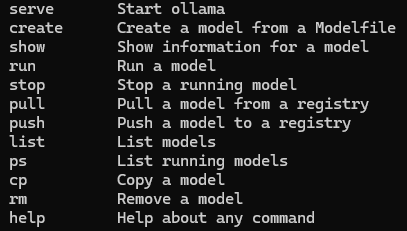
\includegraphics[width=.5\textwidth]{imagenes/0015_ollamaCMD.png}
                \caption{Lista de comandos disponibles de Ollama}
                \label{fig:0015_ollamaCMD}
            \end{figure}

            \noindent Como podemos observar en la figura \ref{fig:0015_ollamaCMD}, para usar un modelo tenemos dos opciones: la primera es descargarlo (\textit{pull}) y después ejecutarlo (\textit{run}), y la segunda es directamente ejecutarlo (\textit{run}), ya que lo descargará automáticamente. El comando \textit{serve} es también muy importante ya que inicia la API de Ollama.

            \noindent Por último, las figuras \ref{fig:0016_ollamaCLI} y \ref{fig:0017_ollamaPY}, muestran dos ejemplos de uso de los modelos: la primera figura muestra la ejecución desde línea de comandos, mientras que la segunda figura, muestra un pequeño programa escrito en \textit{Python} que además usa la librería \textit{LangChain} (sección \ref{sec:LangChain}).

            \begin{figure}[H]
                \centering
                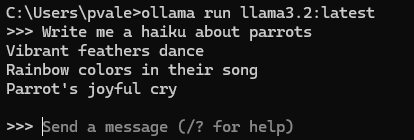
\includegraphics[width=.4\textwidth]{imagenes/0016_ollamaCLI.png}
                \caption{Prueba del CLI de Ollama, ejecuta el modelo \textit{Llama3.2} para hacer una consulta}
                \label{fig:0016_ollamaCLI}
            \end{figure}

            \begin{figure}[H]
                \centering
                \begin{subfigure}{0.49\textwidth}
                    \centering
					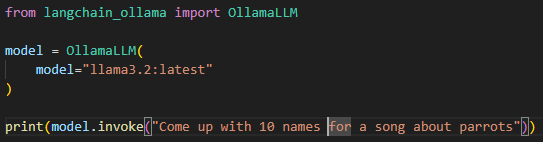
\includegraphics[width=0.9\textwidth]{imagenes/0017_ollamaPY1.png}
					\caption{Código de la aplicación}
                \end{subfigure}   
                \begin{subfigure}{0.49\textwidth}
                    \centering
					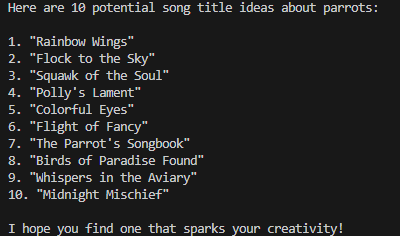
\includegraphics[width=0.9\textwidth]{imagenes/0017_ollamaPY2.png}
					\caption{Resultado de la ejecución}
                \end{subfigure}                  
				\caption{Pequeño programa escrito en \textit{Python}, usando la librería \textit{LangChain}. Pide al modelo \textit{Llama3.2} una consulta}
				\label{fig:0017_ollamaPY}
            \end{figure}
        
        \subsection{Alternativas: LM Studio}
        
            LM Studio \cite{0050_lmstudioDOCS} es aplicación multi-plataforma (\textit{Windows}, \textit{Linux} y \textit{macOS}) en la que podemos usar grandes modelos de lenguaje de forma local, sin conexión a la nube. Es similar a Ollama salvo que esta no es una opción de código abierto y además, cuenta con una interfaz gráfica sencilla e intuitiva (ver figura \ref{fig:0018_lmstudio}).

            \begin{figure}[H]
                \centering
                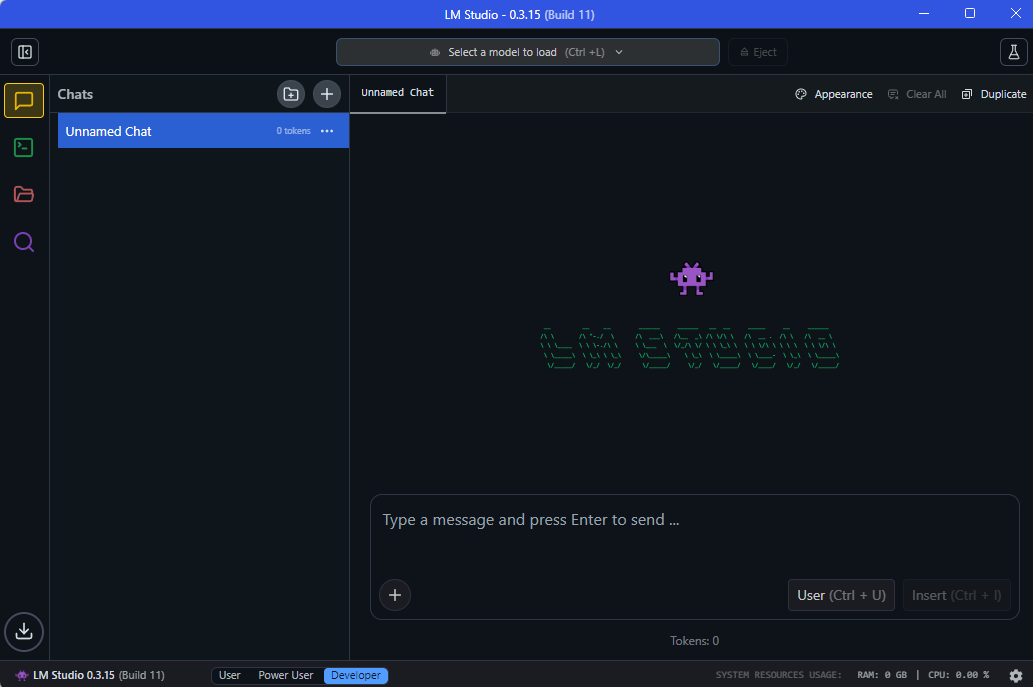
\includegraphics[width=.8\textwidth]{imagenes/0018_lmstudio.png}
                \caption{Pantalla principal de LM Studio, la pestaña activa nos permite chatear con un LLM}
                \label{fig:0018_lmstudio}
            \end{figure}

            \noindent Fijándonos en la figura \ref{fig:0018_lmstudio}, la parte de arriba posee una especie de botón usado para seleccionar y cargar el LLM que deseemos usar (ver figura \ref{fig:0019_lms_load}).

            \begin{figure}[H]
                \centering
                \begin{subfigure}{0.49\textwidth}
                    \centering
					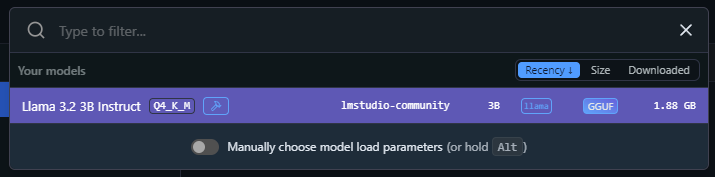
\includegraphics[width=0.9\textwidth]{imagenes/0019a_lms_llm.png}
					\caption{Selección}
                \end{subfigure}   
                \begin{subfigure}{0.49\textwidth}
                    \centering
					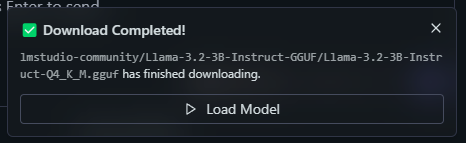
\includegraphics[width=0.9\textwidth]{imagenes/0019b_lms_load.png}
					\caption{Carga}
                \end{subfigure}                  
				\caption{Selección y carga de una versión de \textit{Llama3.2} en LM Studio}
				\label{fig:0019_lms_load}
            \end{figure}

            \noindent Siguiendo en la figura \ref{fig:0018_lmstudio}, la barra de la izquierda dispone de otras tres pestañas (de arriba a abajo):

            \begin{itemize}
                \item \textbf{Developer}: Nos permite activar o desactivar la API de LM Studio (ver figura \ref{fig:0020_lms_api}).
                \item \textbf{My models}: En la cual podemos ver los modelos descargados (figura \ref{fig:0021_lms_models}).
                \item \textbf{Discover}: Permite descargar nuevos modelos (figura \ref{fig:0022_lms_discoverpng}).
            \end{itemize}

            \begin{figure}[H]
                \centering
                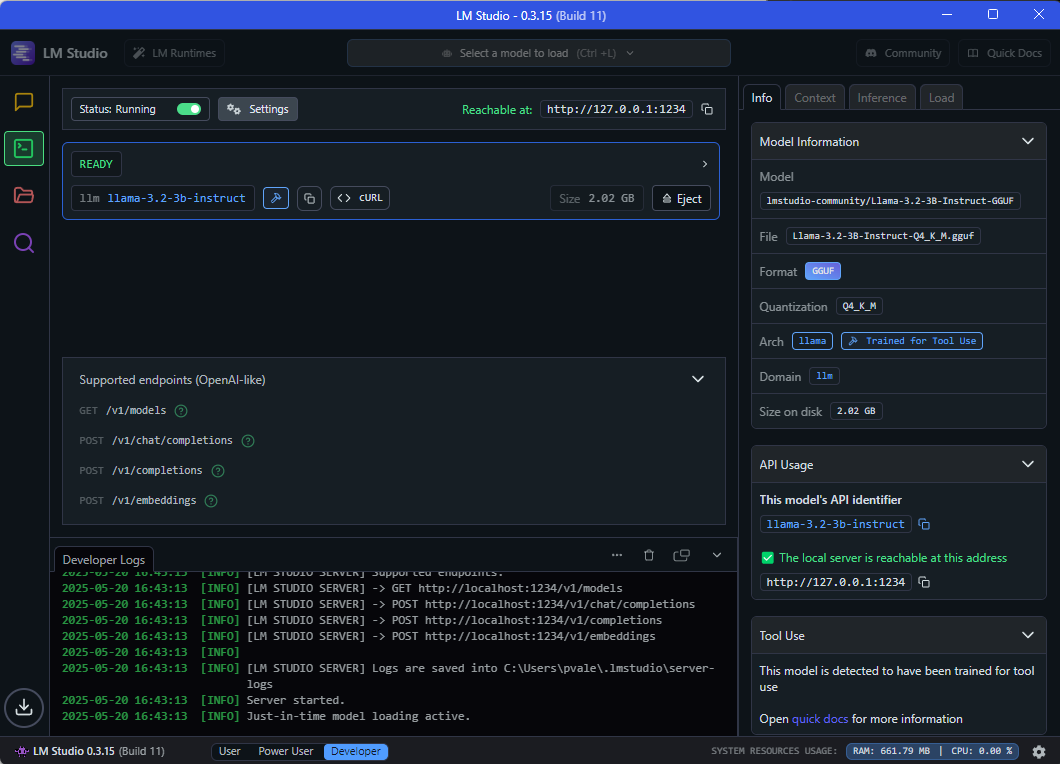
\includegraphics[width=.8\textwidth]{imagenes/0020_lms_api.png}
                \caption{Developer. Pestaña que permite controlar la API de LM Studio, se observa el modelo cargado, la dirección IP de esta y los logs}
                \label{fig:0020_lms_api}
            \end{figure}

            \begin{figure}[H]
                \centering
                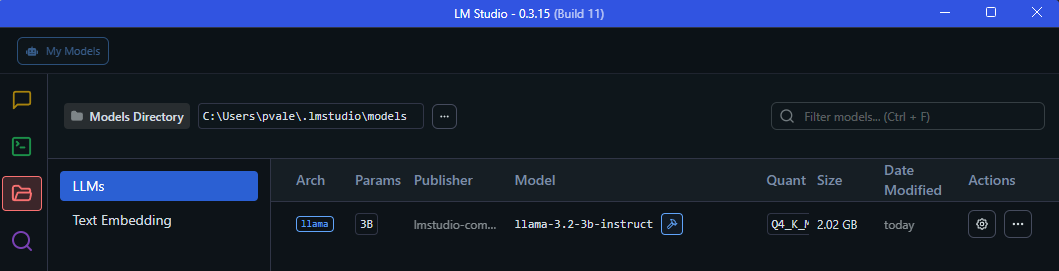
\includegraphics[width=.8\textwidth]{imagenes/0021_lms_models.png}
                \caption{My Models. Pestaña que permite ver los LLMs descargados en LM Studio}
                \label{fig:0021_lms_models}
            \end{figure}

            \begin{figure}[H]
                \centering
                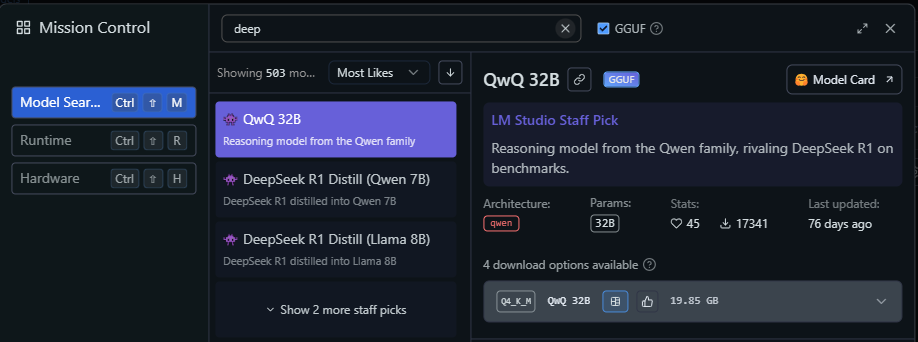
\includegraphics[width=.8\textwidth]{imagenes/0022_lms_discoverpng.png}
                \caption{Discover. Pestaña que permite descargar cualquier LLM disponible en LM Studio}
                \label{fig:0022_lms_discoverpng}
            \end{figure}            

            \subsubsection{Prueba de la API de LM Studio}

                Antes de poder probar la API de LM Studio, es necesario  instalar el paquete \textit{lmstudio} en nuestra instalación de \textit{Python}. Después con un código sencillo como el de la figura \ref{fig:0023_lms_python}, obtenemos una respuesta del LLM cargado previamente. 
                
                \noindent \textbf{Nota:}Aunque no se especifique en el código el LLM que debe usar, utiliza la versión de \textit{Llama3.2} cargada en la API que puede observarse en la figura \ref{fig:0020_lms_api}, en el lateral de de la derecha.
    
                \begin{figure}[H]
                    \centering
                    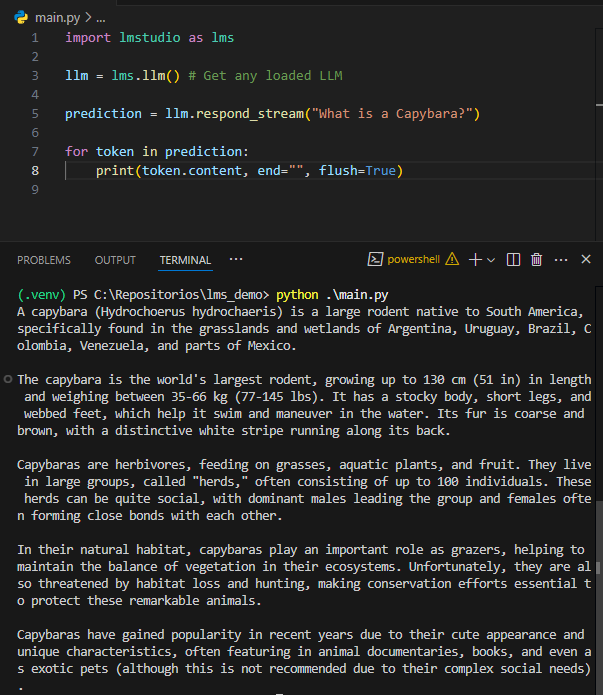
\includegraphics[width=.6\textwidth]{imagenes/0023_lms_python.png}
                    \caption{Pequeño código en Python, para la prueba de la API de LM Studio}
                    \label{fig:0023_lms_python}
                \end{figure}
            
            \subsubsection{Conclusiones: Ollama - LM Studio}

                Ollama y LM Studio presentan dos herramientas potentes para manejar LLMs de forma local. Aunque LM Studio ofrece una interfaz atractiva y sencilla de usar, son las integraciones de este las que dificultan su uso en aplicaciones más avanzadas. 
                
                \noindent Ollama esta pensado para esto último, siendo más sencillo de integrar con librerías externas, ya sean para ayudar en la recuperación de información (ChromaDB \ref{sec:chroma}) o dedicadas al manejo de LLMs (LangChain \ref{sec:LangChain}).

                \noindent Para finalizar, pese a que Ollama no cuenta con una interfaz gráfica, los comandos disponibles para la consola son intuitivos y fáciles de aprender, facilitando su adopción para usuarios menos expertos.

    \section{ChromaDB}
    \label{sec:chroma}

        ChromaDB \cite{0051_chromaDBDOCS} es una base de datos vectorial de código abierto, diseñada para almacenar y recuperar eficientemente vectores de embedding (sección \ref{sec:embeddings}), es decir, las representaciones numéricas de elementos como documentos de texto, imágenes, o vídeos. Su principal función es almacenar estas representaciones vectoriales con una serie de metadatos asociados para su posterior procesado por parte de un LLM. 

        \begin{figure}[H]
            \centering
            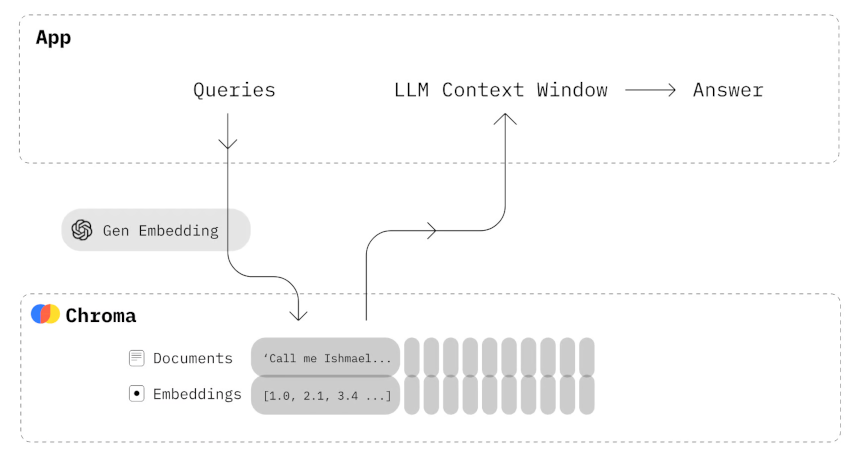
\includegraphics[width=.7\textwidth]{imagenes/0024_chroma.png}
            \caption{Esquema básico del funcionamiento de ChromaDB}
            \label{fig:0024_chroma}
        \end{figure}

        \subsection{Características de ChromaDB}

            ChromaDB posee un conjunto de características que hacen el adecuado para ser la base de datos vectorial de cualquier proyecto \cite{0013_chroma}. La lista siguiente muestra las más importantes:

            \begin{itemize}
                \item \textbf{Simple y potente:} Se instala con un simple comando ``\textit{pip install chromadb}'' y se integra sin problemas mediante la SDK de \textit{Python}, permitiendo una rápida configuración.
                \item \textbf{Multi-función:} Cuenta con una amplia gama de funcionalidades como la búsqueda vectorial, búsqueda de texto, almacenamiento de documentos, filtrado de metadatos, y recuperación multi-modal. Asimismo, es apto para aplicaciones que requieran una alta escalabilidad.
                \item \textbf{Gran soporte de lenguajes:} Ofrece SDKs para los lenguajes de programación más populares, incluyendo \textit{Python}, \textit{JavaScript/TypeScript}, \textit{Ruby}, \textit{PHP} y \textit{Java}.
                \item \textbf{Integración de base:} Cuenta con un enfoque de integración nativo para modelos de embedding de \textit{HuggingFace}, \textit{OpenAI}, \textit{Ollama}, y más. Del mismo modo, es compatible con las librerías \textit{LangChain}, \textit{LlamaIndex}, y muchas más previstas en un futuro.                
                \item \textbf{Almacenamiento local:} Las bases de datos pueden ser almacenadas tanto en memoria como en nuestro equipo local, manteniendo nuestra información privada y no dependiente de servicios externos.
                \item \textbf{Código abierto}: Bajo la licencia Apache2.0.
            \end{itemize}

        \subsection{Funcionamiento de ChromaDB}

            El funcionamiento de esta base de datos es simple y se puede poner en marcha rápidamente utilizando \textit{Python} \cite{014_chromaGS}. En la figura \ref{fig:0025_chromaGS} se muestra un método para crear la base de datos, añadir documentos y realizar consultas (líneas 4, 8 y 16 respectivamente).
    
            \begin{figure}[H]
                \centering
                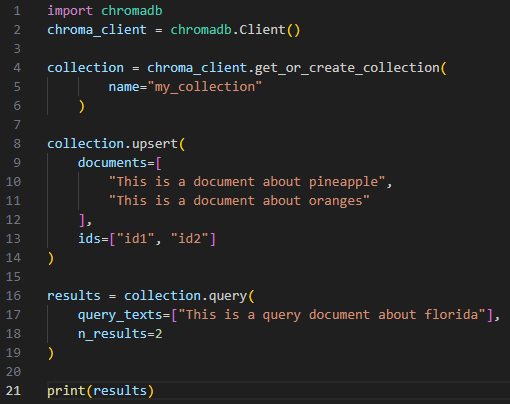
\includegraphics[width=.7\textwidth]{imagenes/0025_chromaGS.png}
                \caption{ChromaDB, puesta en marcha mediante \textit{Python}}
                \label{fig:0025_chromaGS}
            \end{figure}
            
            \noindent Existen varias formas de realizar cada uno de estos pasos. Por ejemplo, al crear el cliente Chroma, podemos especificar el modelo de embedding (por defecto se utiliza \textit{all-MiniLM-L6-v2}).
            
            \noindent En cuanto a la inserción de documentos, cuando la base de datos recibe un texto, lo convierte en su representación vectorial utilizando el modelo de embedding y asocia los metadatos correspondientes en el proceso.
            
            \noindent Finalmente, las consultas también se vectorizan utilizando el mismo modelo (preferiblemente y devuelven los documentos más relevantes mediante una función de búsqueda (por defecto, la similitud coseno).
            
            \noindent Los resultados (figura \ref{fig:0026_chromaGS2}) obtenidos al ejecutar el código mostrado en la figura anterior indican las distancias (línea 10) de los documentos recuperados. Estos resultados representan el output de la búsqueda en la base de datos, donde el documento cuyo ID es ``id2'' tiene una puntuación más alta (menos es mejor).
            
            \begin{figure}[H]
                \centering
                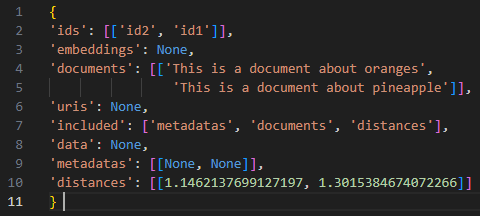
\includegraphics[width=.7\textwidth]{imagenes/0026_chromaGS2.png}
                \caption{ChromaDB. Resultados de la consulta, se observan las distancias de los documentos recuperados}
                \label{fig:0026_chromaGS2}
            \end{figure}            
        
        \subsection{Alternativas: Pinecone}            
            
            Pinecone \cite{0052_pineconeDOCS} es una base de datos vectorial gestionada en la nube \cite{0015_pinecone}, diseñada para realizar búsquedas en tiempo real por similaridad siendo altamente escalable. Esta tecnología ha ganado en popularidad por su facilidad de uso y por su rendimiento.

            \subsubsection{Pros y contras de Pinecone}

                Este modelo de recuperación contiene un conjunto de ventajas similar a ChromaDB con la única excepción del alojamiento web. Veamos algunas de ellas:

                \begin{itemize}
                    \item \textbf{Búsqueda en tiempo real}:  Pinecone ofrece una capacidad de búsqueda asombrosamente rápida, permitiendo a los usuario recuperar vectores similares en tiempo real. 
                    \item \textbf{Escalabilidad}: La arquitectura de Pinecone escala ante un crecimiento de la demanda.
                    \item \textbf{Indexado automático}: Los vectores son indexados automáticamente por Pinecone, reduciendo la carga de trabajo y simplificando el proceso de despliegue.
                    \item \textbf{Soporte Python}: La SDK de \textit{Python} es sencilla de utilizar, haciendo accesible Pinecone para todos los desarrolladores y científicos de datos familiarizados con este ecosistema.
                \end{itemize}

                \noindent Sin embargo, tiene dos inconveniente que podrían ser clave para un proyecto. Uno de ellos es el coste, al ser un servicio en la nube, Pinecone ofrece un modelos de negocio basado en tres tipos de categorías: \textit{Starter} gratuito y pensado para pequeñas aplicaciones, \textit{Standard} para aplicaciones de producción a cualquier escala y \textit{Enterprise} para aplicaciones críticas.

                \noindent La segunda desventaja es la funcionalidad limitada a la hora de realizar consultas avanzadas. A pesar de que Pinecone sobresale en búsquedas por similaridad, podría carecer de algunas capacidades de consulta avanzadas que ciertos proyectos requieren.

            \subsubsection{Funcionamiento de Pinecone}

                Para utilizar Pinecone antes debemos cumplir ciertos requisitos: tenemos que obtener una clave para su API y debemos instalar la SDK de \textit{Python}. La clave nos permite conectar con el servicio web, permitiéndonos crear índices (ver figuras \ref{fig:0028_pinecone1}, \ref{fig:0029_pinecone2} y \ref{fig:0029_pinecone21}) y enviar documentos (figuras \ref{fig:0030_pinecone3} y \ref{fig:0030_pinecone31}). 

                \begin{figure}[H]
                    \centering
                    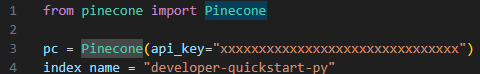
\includegraphics[width=.6\textwidth]{imagenes/0028_pinecone1.png}
                    \caption{Pinecone. Inicialización a través de su clave API}
                    \label{fig:0028_pinecone1}
                \end{figure} 

                \begin{figure}[H]
                    \centering
                    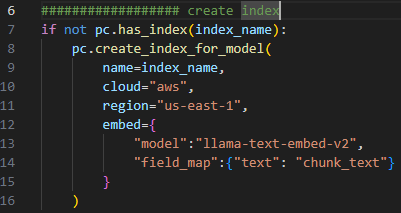
\includegraphics[width=.6\textwidth]{imagenes/0029_pinecone2.png}
                    \caption{Pinecone. Creación de un índice}
                    \label{fig:0029_pinecone2}
                \end{figure} 

                \begin{figure}[H]
                    \centering
                    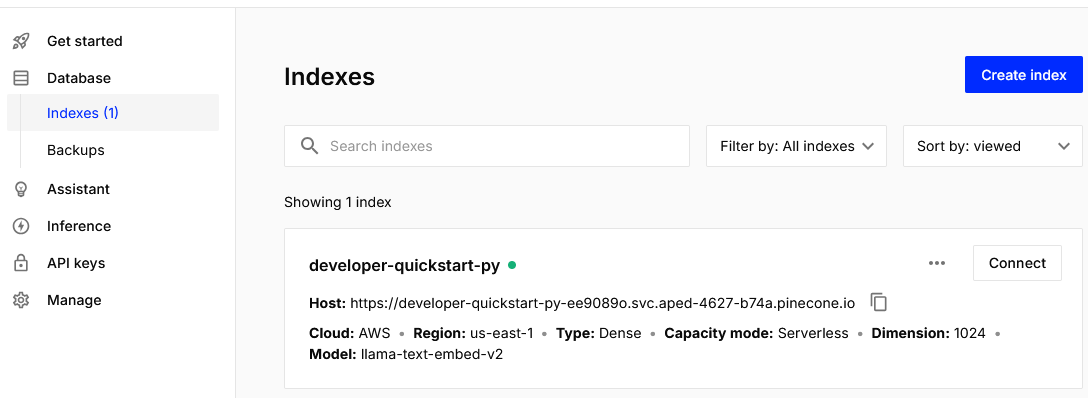
\includegraphics[width=.8\textwidth]{imagenes/0029_pinecone2-1.png}
                    \caption{Pinecone. Vista del índice en la web}
                    \label{fig:0029_pinecone21}
                \end{figure}     

                \begin{figure}[H]
                    \centering
                    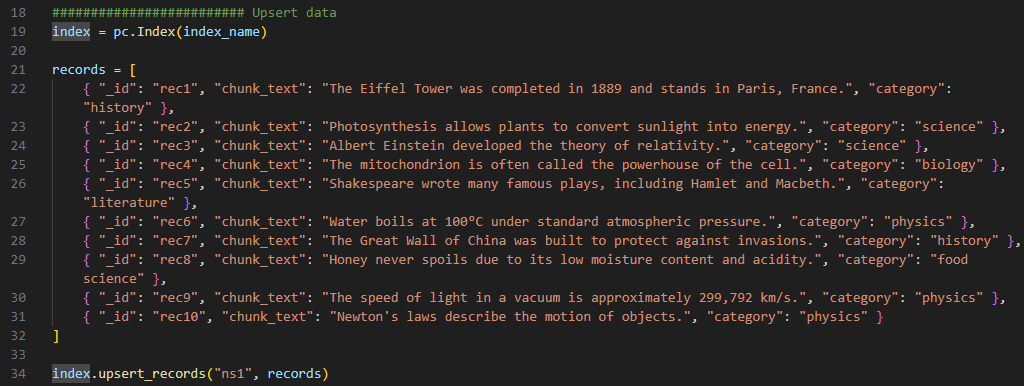
\includegraphics[width=.8\textwidth]{imagenes/0030_pinecone3.png}
                    \caption{Pinecone. Agregación de documentos}
                    \label{fig:0030_pinecone3}
                \end{figure} 

                \begin{figure}[H]
                    \centering
                    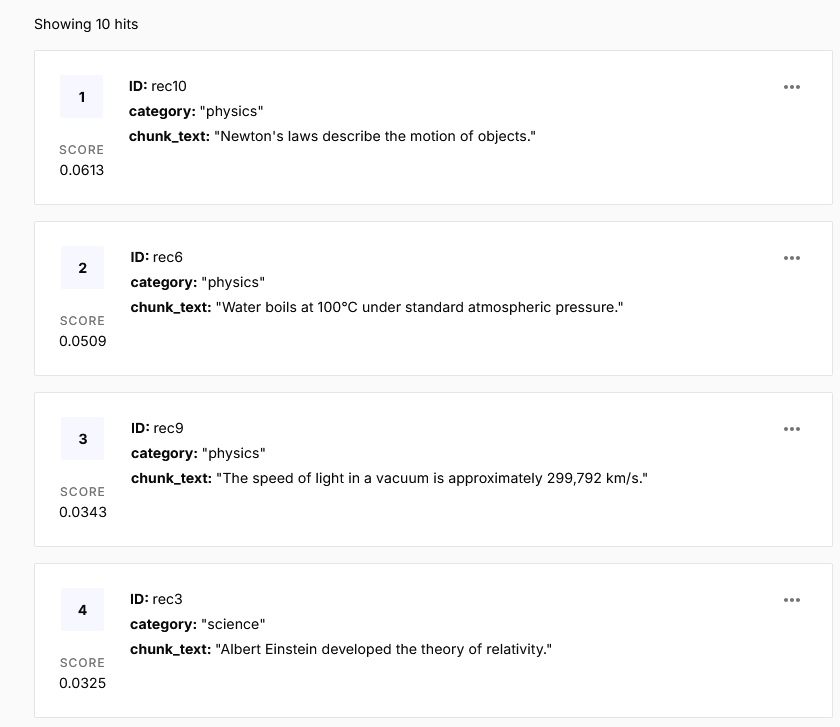
\includegraphics[width=1\textwidth]{imagenes/0030_pinecone3-1.png}
                    \caption{Pinecone. Vista de documentos en la web}
                    \label{fig:0030_pinecone31}
                \end{figure}        

                \noindent Las búsquedas en Pinecone se pueden realizar como se muestra en la siguiente figura: especificando la consulta y los parámetros de recuperación deseados (ver figura \ref{fig:0031_pinecone}). Pinecone ofrece también la posibilidad de hacer \textit{rerank} a los resultados (véase la figura \ref{fig:0032_pinecone}), es decir, un refinamiento o re-ordenación de los documentos recuperados basado en la relevancia ante una consulta.

                \begin{figure}[H]
                    \centering
                    \begin{subfigure}{0.49\textwidth}
                        \centering
    					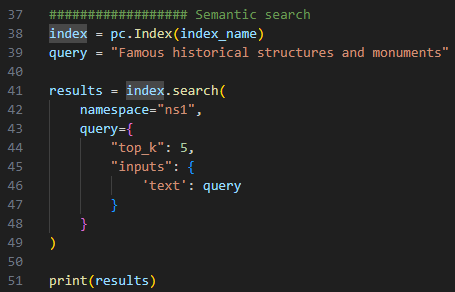
\includegraphics[width=0.9\textwidth]{imagenes/0031_pinecone4.png}
    					\caption{Búsqueda semántica}
                    \end{subfigure}   
                    \begin{subfigure}{0.49\textwidth}
                        \centering
    					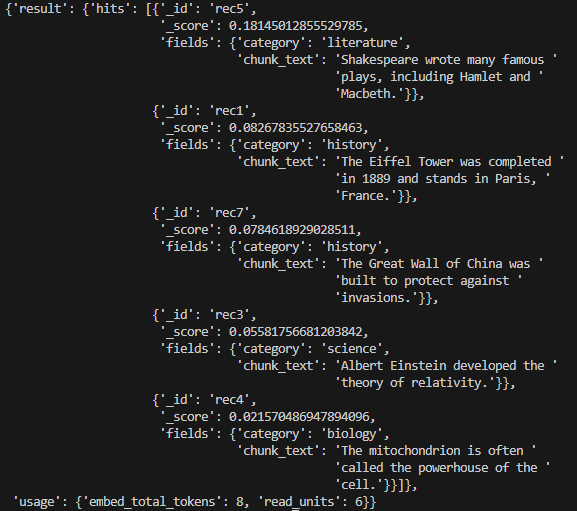
\includegraphics[width=0.9\textwidth]{imagenes/0031_pinecone5.png}
    					\caption{Resultados}
                    \end{subfigure}                  
    				\caption{Pinecone. Búsqueda semántica y resultados}
    				\label{fig:0031_pinecone}
                \end{figure}

                \begin{figure}[H]
                    \centering
                    \begin{subfigure}{0.49\textwidth}
                        \centering
    					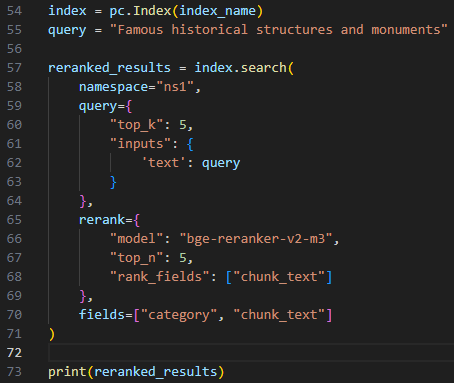
\includegraphics[width=0.9\textwidth]{imagenes/0032_pinecone6.png}
    					\caption{Reranking}
                    \end{subfigure}   
                    \begin{subfigure}{0.49\textwidth}
                        \centering
    					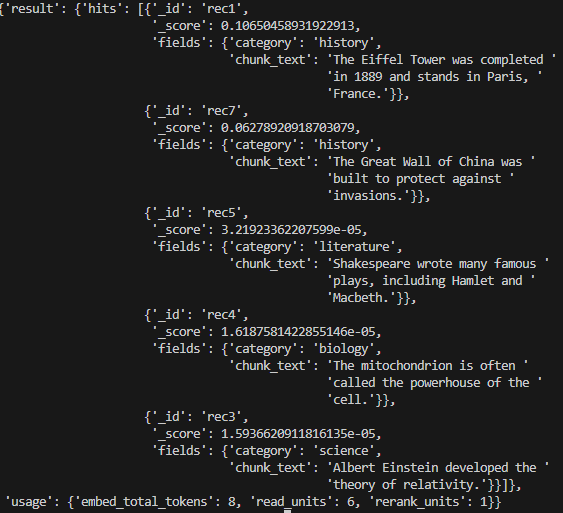
\includegraphics[width=0.9\textwidth]{imagenes/0032_pinecone7.png}
    					\caption{Resultados}
                    \end{subfigure}                  
    				\caption{Pinecone. Reranking y resultados}
    				\label{fig:0032_pinecone}
                \end{figure}

                \noindent Se puede observar una clara diferencia entre los resultados de las dos últimas figuras, siendo los obtenidos aplicando \textit{reranking} mucho más relevantes respecto a la consulta hecha.

            \subsubsection{Conclusión sobre Pinecone}
                
                Tras analizar el funcionamiento, características y diferencias entre ChromaDB y Pinecone, se puede concluir que ChromaDB representa una opción superior para muchos escenarios de desarrollo, especialmente aquellos en los que la privacidad, el control total sobre los datos y la independencia de servicios externos son prioritarios.

                \noindent La principal ventaja de ChromaDB reside en su capacidad para operar de manera local, sin necesidad de conexión a la nube. Esta característica permite que la información sensible se mantenga en el entorno del usuario, eliminando preocupaciones relacionadas con la exposición de datos o la dependencia de terceros. Además, su instalación sencilla, su compatibilidad con múltiples lenguajes y herramientas, y su naturaleza de código abierto lo convierten en una solución robusta y versátil para sistemas de recuperación de información basados en embeddings.
                
                \noindent Si bien Pinecone ofrece una infraestructura escalable y tiempos de respuesta rápidos, su condición de servicio en la nube introduce limitaciones importantes en términos de coste, privacidad y flexibilidad. Por tanto, para proyectos que requieran control local, transparencia y personalización, ChromaDB se posiciona como la alternativa preferente.

    \section{LangChain}
    \label{sec:LangChain}

        LangChain \cite{0053_langchainDOCS} se ha convertido en uno de los proyectos de código abierto con más rápido crecimiento en la historia, debido en gran medida al creciente interés surgido en al ámbito de los LLMs \cite{0016_langchain}. LangChain es un framework centrado en el desarrollo de aplicaciones impulsadas por los grandes modelos de lenguaje, cubriendo cada etapa de la vida de la aplicación: desde el desarrollo usando componentes de código abierto de LangChain o integraciones de terceros, la producción con la herramienta inspectora \textit{LangSmith}, y el despliegue a través de \textit{LangGraph}.

        \noindent LangChain implementa una interfaz estandar para los LLMs y tecnologías relacionadas, como son los modelos de embedding y las bases de datos vectoriales, y esta integrado con cientos de proveedores.

        \begin{figure}[H]
            \centering
            \includegraphics[width=.6\textwidth]{imagenes/0033_LangChain1.jpg}
            \caption{Esquema que muestra las diferentes aplicaciones en las que podemos usar LangChain \cite{0017_langchain2}}
            \label{fig:0033_LangChain1}
        \end{figure} 

        \noindent La importancia de LangChain radica en un conjunto de factores. El primero de ellos es que simplifica el proceso de desarrollo, reduciendo la complejidad a la hora de construir aplicaciones LLM por medio de plantillas estructuradas. Esto permite a los desarrolladores hacer las aplicaciones de manera modular, haciendo que sean más fáciles de manejar y escalar.

        \noindent A parte, LangChain permite la integración con múltiples LLMs, permitiéndonos usar el que más nos apetezca. Por último, el sistema de ``\textit{chaining}'' (o encadenamiento) ofrece una forma eficiente de llamar a los modelos, lo que incrementa el rendimiento y la precisión de la aplicación \cite{0017_langchain2}.

        \subsection{Características e integraciones de LangChain}

            Aunque ya hemos comentado algunas de las características o integraciones de LangChain, a continuación comentaremos algunas de las más importantes que tiene.

            \subsubsection{Características}

                \begin{itemize}
                    \item \textbf{Diseño modular:} Divide el proceso de desarrollo en módulos manejables, cada uno, asumiendo un aspecto específico de la aplicación.
                    \item \textbf{Manejo del prompt:} Provee de herramientas para crear y manejar prompts de manera eficiente.
                    \item \textbf{Chaining:} Permite enlazar múltiples prompts y modelos para crear flujos de trabajo complejos.
                    \item \textbf{Manejo del output:} Facilita el post-procesado de la salida de los modelos proporcionando una mejor usabilidad.
                \end{itemize}

            \subsubsection{Integraciones}    

                \begin{itemize}
                    \item \textbf{OpenAI GPT:} Una de las librerías de LLMs más usadas para el procesado del lenguaje natural.
                    \item \textbf{Mistral AI:} Un LLM desarrollado por la empresa del mismo nombre, diseñada para proporcionar información precisa y asistencia en una variedad de temas.
                    \item \textbf{Ollama:} Una biblioteca donde podemos encontrar una gran cantidad de LLMs de libre acceso.
                    \item \textbf{Hugging Face Transformers:} Una librería que da acceso a un gran número de modelos pre-entrenados.
                    \item \textbf{ChromaDB:} La base de datos vectorial usada en el proyecto.
                \end{itemize}

            \subsection{Tutorial básico de LangChain}

                Las siguientes figuras muestran una pequeña aplicación hecha usando LangChain y el resultado de su ejecución. En la figura \ref{fig:0034_langchain2} podemos ver el diseño modular y las integraciones antes mencionadas que tiene esta herramienta. Podemos observar también el diseño sencillo y sin complicaciones que ofrece a la hora de manejar prompts e integraciones con LLMs.

                \begin{figure}[H]
                    \centering
                    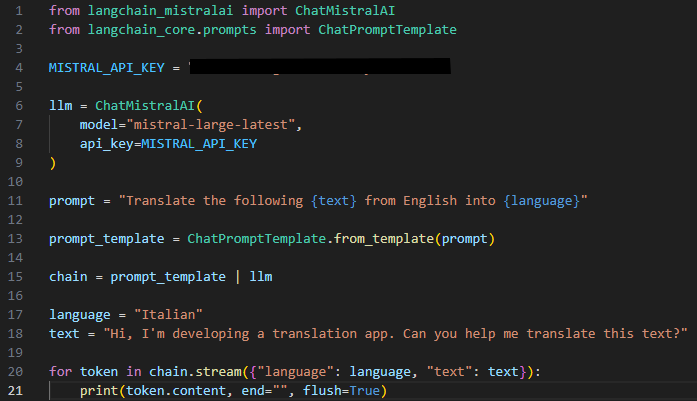
\includegraphics[width=.8\textwidth]{imagenes/0034_langchain2.png}
                    \caption{LangChain. Aplicación sencilla que usa mistral-large (LLM desarrollado por MistralAI) para traducir un texto}
                    \label{fig:0034_langchain2}
                \end{figure}    

                \begin{figure}[H]
                    \centering
                    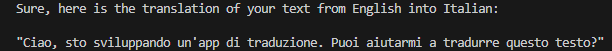
\includegraphics[width=.8\textwidth]{imagenes/0035_langchain3.png}
                    \caption{LangChain. Resultado de la traducción del texto de la figura \ref{fig:0034_langchain2}}
                    \label{fig:0035_langchain3}
                \end{figure}    
        
        \subsection{Alternativas: LlamaIndex}

            LlamaIndex \cite{0054_llamaindexDOCS} es la principal alternativa que tenemos a LangChain. LlamaIndex es un framework que simplifica la integración de datos públicos y privados en la construcción de aplicaciones usando grandes modelos de lenguaje \cite{0018_llamaindex}. Provee de funcionalidades para ingestar datos, indexación de datos, herramientas de búsqueda, etc, por lo tanto, es una solución muy versátil para construir un RAG.         

            \subsubsection{Funcionalidades principales y beneficios de LlamaIndex}

                El modo de operar de LlamaIndex se puede dividir en tres grandes bloques: ingestión, indexado y consulta \cite{0019_llamaindex2}.

                \noindent En la ingesta de datos, LlamaIndex simplifica el proceso de conectar con datos externos, desde APIs, PDFs o bases de datos. Esto asegura que datos con o sin estructura puedan ser integrados en aplicaciones LLM.

                \noindent Una vez los datos son ingestados, LlamaIndex dispone de múltiples modelos de indexación para representar datos de manera eficiente. Alguna de estas herramientas son:

                \begin{itemize}
                    \item \textbf{List Index}: Organizan los datos secuencialmente, apto para objetos estructurados que cambian en el tiempo.
                    \item \textbf{Tree Index}: Estructura los datos en forma de árbol.
                    \item \textbf{Vector Store Index}: Almacena los datos provenientes de un modelo de embedding, facilitando al vector hacer búsquedas por similaridad.
                    \item \textbf{keyword Index}: Asocia los metadatos a los datos almacenados.
                \end{itemize}

                \noindent Por último, a la hora de consultar, LlamaIndex aprovecha el procesado del lenguaje natural que posee para facilitar dichas consultas a través de un prompt. Este enfoque permite a los usuarios interactuar con los datos usando su propio lenguaje natural, simplificando el proceso de recuperación de información

            \subsubsection{Diferencias en el código: LangChain vs LlamaIndex}           
                A continuación mostraremos algunas figuras comparativas, donde veremos el código de LangChain y LlamaIndex para hacer una misma función.

                \begin{figure}[H]
                    \centering
                    \begin{subfigure}{0.49\textwidth}
                        \centering
    					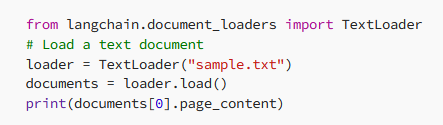
\includegraphics[width=1\textwidth]{imagenes/0037_loaders1.png}
    					\caption{LangChain}
                    \end{subfigure}   
                    \begin{subfigure}{0.49\textwidth}
                        \centering
    					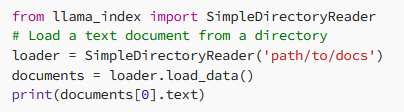
\includegraphics[width=1\textwidth]{imagenes/0037_loaders2.png}
    					\caption{LlamaIndex}
                    \end{subfigure}                  
    				\caption{Loaders, se encarga de cargar documentos \cite{0020_llamaindex3}}
    				\label{fig:0037_loaders}
                \end{figure}

                \begin{figure}[H]
                    \centering
                    \begin{subfigure}{0.49\textwidth}
                        \centering
    					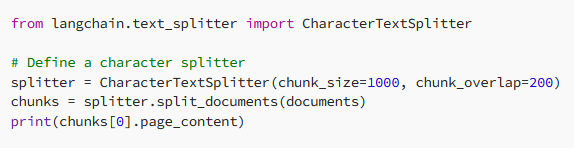
\includegraphics[width=1\textwidth]{imagenes/0038_splitters1.png}
    					\caption{LangChain}
                    \end{subfigure}   
                    \begin{subfigure}{0.49\textwidth}
                        \centering
    					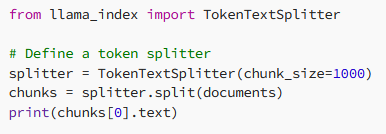
\includegraphics[width=1\textwidth]{imagenes/0038_splitters2.png}
    					\caption{LlamaIndex}
                    \end{subfigure}                  
    				\caption{Splitter, se encarga de trocear los documentos \cite{0020_llamaindex3}}
    				\label{fig:0038_splitters}
                \end{figure}

                \noindent Podemos apreciar en las figuras \ref{fig:0037_loaders} y \ref{fig:0038_splitters}, que la forma que tienen ambas herramientas de cargar y separar documentos es similar, usando sendas funciones con las que obtienen el mismo resultado.

                \begin{figure}[H]
                    \centering
                    \begin{subfigure}{0.49\textwidth}
                        \centering
    					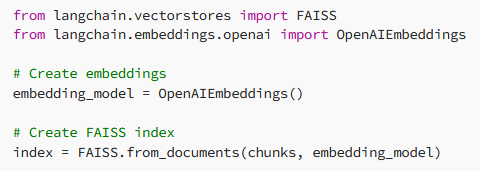
\includegraphics[width=1\textwidth]{imagenes/0039_indexing1.png}
    					\caption{LangChain}
                    \end{subfigure}   
                    \begin{subfigure}{0.49\textwidth}
                        \centering
    					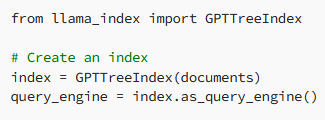
\includegraphics[width=1\textwidth]{imagenes/0039_indexing2.png}
    					\caption{LlamaIndex}
                    \end{subfigure}                  
    				\caption{Indexing, se encarga de almacenar los documentos en la base de datos vectorial \cite{0020_llamaindex3}}
    				\label{fig:0039_indexing}
                \end{figure}

                \noindent En cambio, la figura anterior muestra una diferencia. Por un lado, LangChain muestra su capacidad de integración personalizando los modelos de embedding y la base de datos a usar, mientras que LlamaIndex simplifica este proceso creando una estructura jerárquica y usando valores por defecto.

                \begin{figure}[H]
                    \centering
                    \begin{subfigure}{0.49\textwidth}
                        \centering
    					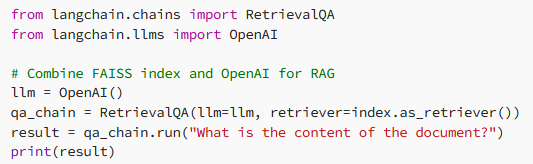
\includegraphics[width=1\textwidth]{imagenes/0040_chains1.png}
    					\caption{LangChain}
                    \end{subfigure}   
                    \begin{subfigure}{0.49\textwidth}
                        \centering
    					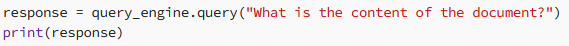
\includegraphics[width=1\textwidth]{imagenes/0040_chains2.png}
    					\caption{LlamaIndex}
                    \end{subfigure}                  
    				\caption{Chains/Query, se encarga de hacer una consulta a la base de datos vectorial \cite{0020_llamaindex3}}
    				\label{fig:0040_chains}
                \end{figure}

                \noindent A la hora de hacer consultas pasa algo similar a lo visto en la figura \ref{fig:0039_indexing}. La figura \ref{fig:0040_chains} muestra la forma de hacer una consulta con ambas herramientas, siendo mas simple la manera que ofrece LlamaIndex.               
            
            \subsubsection{Conclusión: LangChain vs LlamaIndex}

                Tras evaluar ambas herramientas, se ha determinado que LangChain es la opción más adecuada para el desarrollo de aplicaciones avanzadas basadas en LLMs. 
                
                \noindent LangChain destaca por su excepcional flexibilidad y capacidad de integración, permitiendo un control granular sobre cada componente del flujo de trabajo. Su capacidad para manejar flujos de trabajo multi-modales y su soporte para una amplia gama de modelos y bases de datos vectoriales lo posiciona como una herramienta poderosa para aplicaciones que demandan un alto nivel de personalización. Además, ofrece una interfaz estandarizada, que facilita la integración con multitud de proveedores y simplifica el proceso de desarrollo.
                
                \noindent Aunque LlamaIndex ofrece una solución más sencilla y directa, especialmente adecuada para proyectos que se centran en la recuperación y el procesamiento de documentos estructurados de manera jerárquica, su enfoque simplificado y facilidad de configuración no son suficientes para proyectos que requieren un alto nivel de personalización y control. LangChain, por otro lado, proporciona una infraestructura robusta y versátil que puede adaptarse a una amplia variedad de necesidades y complejidades del proyecto.
                
                \noindent Por lo tanto, LangChain se presenta como la opción superior para aquellos que buscan una solución altamente personalizable y con capacidad de manejar múltiples tipos de datos y estrategias de recuperación complejas. Su capacidad para integrarse con una amplia variedad de modelos y sistemas de almacenamiento, junto con su diseño modular y herramientas avanzadas para el manejo de prompts y outputs, lo convierten en la elección ideal para el desarrollo de aplicaciones avanzadas basadas en LLMs.
            
    \section{Streamlit}
    \label{sec:2_streamlit}

        Streamlit \cite{0055_streamlitDOCS} es un framework de código abierto en Python pensado para desarrollar aplicaciones interactivas basadas en el aprendizaje automático, inteligencia artificial o ciencia de datos. Streamlit permite a los desarrolladores y científicos de datos crear aplicaciones atractivas, informativas o realizar visualizaciones de datos en pocas líneas de código.

        \noindent Una de las principales aspectos de Streamlit es su simpleza y facilidad de aprendizaje. Además, Streamlit dispone de una amplia gama de herramientas o \textit{widgets} de visualización de datos: gráficas, histogramas, mapas, etc \cite{0022_streamlit2}.

        \noindent Otra ventaja de Streamlit es su flexibilidad, permitiendo desarrollar aplicaciones para un gran rango de casos de uso: desde simples código para visualizar datos, hasta aplicaciones complejas basadas en modelos de lenguaje.

        \subsection{Funcionalidades clave de Streamlit}

            Ya hemos mencionado algunos de sus aspectos más importantes, en la siguiente lista mostraremos los aspectos clave que hacen de Streamlit una de las herramientas más potentes \cite{0021_streamlit1}:

            \begin{itemize}
                \item \textbf{Desarrollo centrado en Python}: En contraste con los frameworks web tradicionales, esta herramienta usa Python. Elimina el requerimiento de usar lenguajes orientados a la web.
                \item \textbf{Widgets interactivos}: Como ya hemos comentado, Streamlit dispone de \textit{widgets} propios incluyendo botones, paneles desplegables, etc; que proporcionan más interactividad.
                \item \textbf{Actualizaciones en tiempo real}: Las aplicaciones Streamlit ejecutan el código de Python de arriba hacia abajo, actualizandose automáticamente cada vez que el usuario interactúa con un \textit{widget} o modifica una entrada de datos.
                \item \textbf{Soporte a la visualización de datos}: Streamlit esta integrado con las librerías de visualización de datos más comunes, incluyendo \textit{Seaborn} o \textit{Plotly}.
                \item \textbf{Prototipado rápido}: Streamlit posee una sintaxis sencilla, posibilitando un desarrollo de prototipos ágil y perfeccionamiento posterior.
                \item \textbf{De código abierto y extensible}: Al tener este enfoque, Streamlit confiere a los usuarios la posibilidad de extender su funcionalidad a través de plugins o integraciones hechos por la comunidad.
                \item \textbf{Opciones de despliegue}: Las aplicaciones desarrolladas en Streamlit pueden ser desplegadas en distintas plataformas como: Streamlit Community Cloud, Heroku, o AWS.
            \end{itemize}

        \subsection{Ejemplo de aplicación LLM en Streamlit}

            El siguiente ejemplo muestra una manera sencilla de integrar un LLM en Streamlit, usando varias librerías de LangChain, así como integraciones para los LLMs de Mistral AI y funcionalidades propias de Streamlit.

            \noindent En el caso de uso escogido para el ejemplo, simularemos una conversación con un agente IA que es un asistente de venta de vehículos. Para ello necesitaremos configurar un prompt donde recogeremos las instrucciones que deberá seguir el LLM en su respuesta. La siguiente figura muestra el prompt usado en la aplicación, y además, cuenta con dos variables, la consulta del usuario y el historial de la conversación. De esta manera podemos lograr que nuestro agente tenga memoria, lo que es muy útil en casos como este.
            
            \begin{figure}[H]
                \centering
                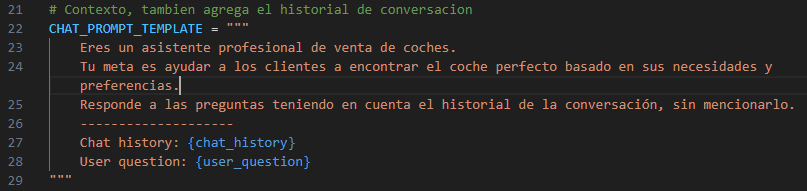
\includegraphics[width=.8\textwidth]{imagenes/0042_streamlit_ejemplo1.png}
                \caption{Ejemplo aplicación LLM en Streamlit. Prompt con dos varitables}
                \label{fig:0042_streamlit_ejemplo1}
            \end{figure}  

            \noindent Como hemos mencionado anteriormente, para este ejemplo hemos usado un LLM perteneciente a Mistral AI, en concreto, ``mistral-small'', dado a que es bastante rápido y eficiente. La figura \ref{fig:0043_streamlit_ejemplo2} muestra como se hace la llamada al LLM usando las herramientas que nos facilita LangChain, acabando retornando la ``chain'' o cadena en la que se escribirá la respuesta.
            
            \begin{figure}[H]
                \centering
                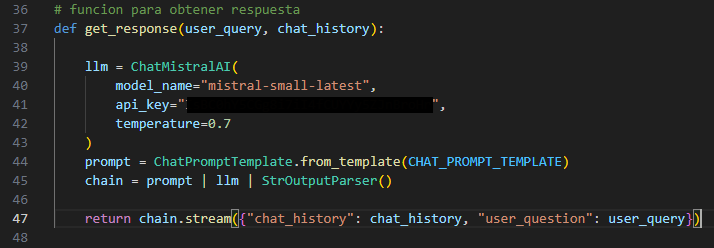
\includegraphics[width=.8\textwidth]{imagenes/0043_streamlit_ejemplo2.png}
                \caption{Ejemplo aplicación LLM en Streamlit. Llamada al LLM}
                \label{fig:0043_streamlit_ejemplo2}
            \end{figure}       

            \noindent El programa principal reflejado en la figura \ref{fig:0044_streamlit_ejemplo3}, no requiere de más de 20 líneas. Si nos fijamos en la línea 58, podemos observar como Streamlit gestiona las sesiones de estado para guardar el historial de conversación. Estas son variables especiales donde podemos guardar el valor de cualquier variable o clase.            

            \noindent La consulta de usuario se guarda fácilmente mediante el método \textit{chat\_input} de Streamlit, que crea en la interfaz un input para la entrada de texto. En las líneas 70 y 75 de figura \ref{fig:0044_streamlit_ejemplo3} podemos ver como se agregan la consulta y la respuesta del modelo a la variable que guarda el historial de conversación, mientras que en la 74, se hace una llamada a la función que retorna la respuesta del modelo. En concreto, el método \textit{write\_stream} de Streamlit escribe la respuesta en tiempo real según van llegando los \textit{tokens} del modelo de lenguaje, proporcionando una respuesta inmediata y una mejor experiencia de usuario.
            
            \begin{figure}[H]
                \centering
                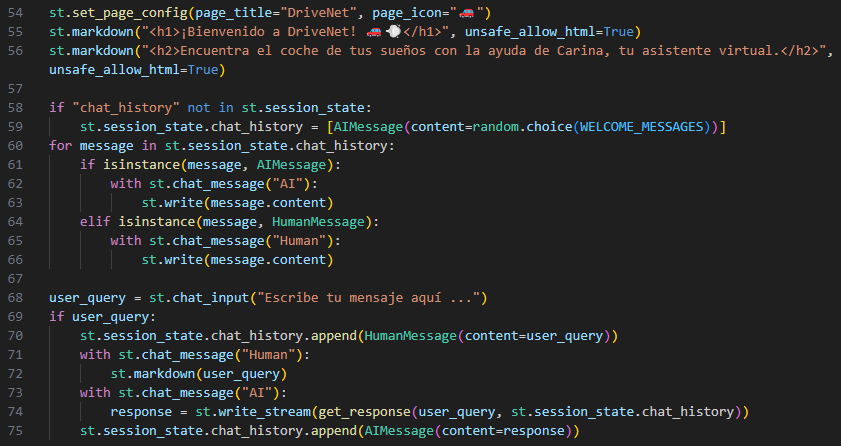
\includegraphics[width=1\textwidth]{imagenes/0044_streamlit_ejemplo3.png}
                \caption{Ejemplo aplicación LLM en Streamlit. Programa principal}
                \label{fig:0044_streamlit_ejemplo3}
            \end{figure}  

            \noindent En resumen, Streamlit se caracteriza por la sencillez de su código y por la integración que permite con otras herramientas como LangChain, etc. La siguiente subsección, muestra algunas capturas del funcionamiento de este ejemplo.

        \subsubsection{Funcionamiento del ejemplo}

            \begin{figure}[H]
                \centering
                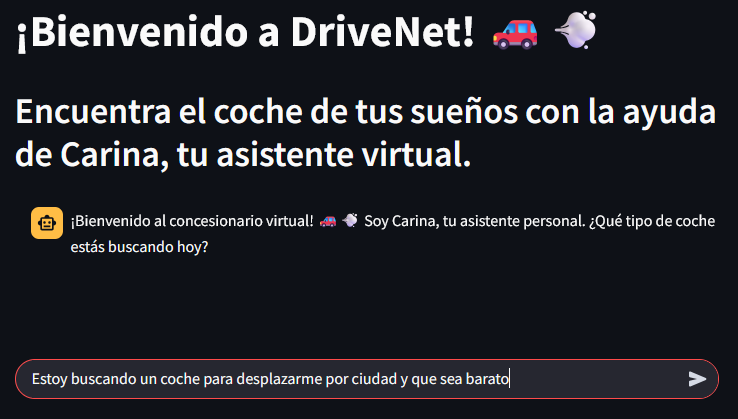
\includegraphics[width=.65\textwidth]{imagenes/0045_ejem1.png}
                \caption{Interfaz del ejemplo aplicación LLM en Streamlit. Bienvenida}
                \label{fig:0045_ejem1}
            \end{figure} 

            \begin{figure}[H]
                \centering
                
\includegraphics[width=.65\textwidth]{imagenes/0046_ejem2.png}
                \caption{Interfaz del ejemplo aplicación LLM en Streamlit. Opciones}
                \label{fig:0046_ejem2}
            \end{figure} 

            \begin{figure}[H]
                \centering
                
\includegraphics[width=.65\textwidth]{imagenes/0047_ejem3.png}
                \caption{Interfaz del ejemplo aplicación LLM en Streamlit. Respuesta con memoria}
                \label{fig:0047_ejem3}
            \end{figure} 
            
    \section{Aplicaciones alternativas al proyecto propuesto}
    
    	En esta sección hablaremos de aplicaciones o servicios similares a nuestro proyecto, aplicaciones de ayuda a ciudadanos ante una catástrofe natural, como la DANA; o servicios que usen de base un RAG para facilitar el acceso a la información. 
    	
    	\subsection{Ajuda Dana}
    	
    		Ajuda Dana \cite{0057_ajudana2} es una plataforma digital colaborativa creada tras la DANA en Valencia para coordinar de forma centralizada la ayuda a los afectados. Nació el 31 de octubre de 2024 a partir de la unión de iniciativas espontáneas en redes sociales, y que reunió a voluntarios de diferentes perfiles (informáticos, logísticos, atención al cliente, etc.), organizados como si fueran una empresa, pero sin apoyo oficial \cite{0057_ajudana}.
    		
    		\begin{figure}[H]
    			\centering
    			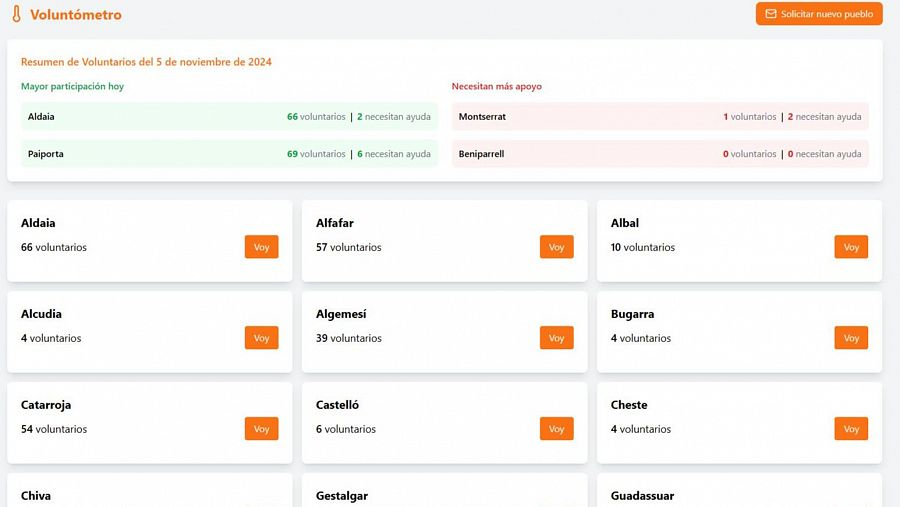
\includegraphics[width=.8\textwidth]{imagenes/0150_ajudana.jpg}
    			\caption{El voluntómetro muestra las solicitudes de ayuda y los voluntarios que hay en cada lugar \cite{0057_ajudana}}
    			\label{fig:0150_ajudana}
    		\end{figure} 
    		
    		\noindent La aplicación conecta solicitudes de ayuda con ofertas de voluntariado, gestionando peticiones y ofrecimientos en tareas como limpieza, alojamiento, asistencia médica, apoyo psicológico o transporte. Además, integra un servicio de búsqueda de desaparecidos, con el que han logrado localizar a 20 personas \cite{0057_ajudana}.
    		
    		\noindent Entre sus funcionalidades destacan:
    		
    		\begin{itemize}
    			\item Registro de solicitudes con niveles de urgencia (rojo, naranja, verde).
    			\item Mapa de puntos de recogida y distribución de suministros.
    			\item Teléfono gratuito para personas mayores sin acceso a internet.
    			\item Validación de información para evitar datos falsos.
    		\end{itemize}
    		
    		\noindent Ajuda Dana se ha convertido en una herramienta clave de coordinación ciudadana, combinando tecnología, voluntariado y solidaridad para dar respuesta rápida y eficaz a una emergencia colectiva.
    		
    	\subsection{TuCocheDana}
    	
    		TuCocheDANA era una plataforma digital creada durante la DANA para ayudar a propietarios a recuperar sus vehículos perdidos tras las riadas. La iniciativa fue desarrollada por Juan Francisco Soler, profesor de informática en el IES Alyanub de Almería, y su exalumno René Molina, estudiante de Ingeniería Mecánica en la UPV \cite{0058_tucochedana}.
    		
    		\noindent Su funcionamiento era sencillo:
    		
    		\begin{itemize}
    			\item Si una persona encontraba un coche abandonado, podía registrarlo indicando matrícula, ubicación, marca, color y detalles adicionales.
    			\item Si otra persona buscaba su coche perdido, bastaba introducir la matrícula en el buscador para obtener información y la localización exacta.
    		\end{itemize}   		
    		
    		\noindent La plataforma garantizaba la privacidad no proporcionando un listado abierto de coches encontrados, tan solo mostraba los datos vinculados a la matrícula introducida. Además, a través de un bot de Telegram, avisaba automáticamente a los propietarios cuando su coche fuese registrado, evitando así que tuviesen que comprobar la web de forma constante \cite{0058_tucochedana}.
    		
    		\noindent La plataforma funcionaba a través de la web tucochedana.es, que actualmente esta cerrada debido al tiempo transcurrido desde la tragedia.
    		
    		\noindent En resumen, TuCocheDANA fué un ejemplo de innovación digital solidaria, que combinó tecnología, colaboración ciudadana y gestión responsable de datos para resolver un problema muy concreto tras la catástrofe.
    		
    	\subsection{Justicio}
    	
	    	Justicio \cite{0060_justicio} es una plataforma de código abierto que utiliza un enfoque RAG, combinando la API de \textit{OpenAI} con la base de datos vectorial \textit{Qdrant}. Gracias a esta arquitectura, es capaz de entender consultas en lenguaje natural, recuperar información legislativa relevante y generar respuestas claras y fundamentadas, citando siempre las fuentes originales \cite{0060_justicio2}.
	    	
	    	\noindent Inicialmente concebido como un chatbot jurídico, Justicio se entrenó con legislación estatal, autonómica y europea, permitiendo a cualquier persona —desde juristas hasta ciudadanos sin formación legal— acceder de manera rápida y comprensible a normativas complejas. Su valor diferencial radica en transformar el BOE y otros textos legales densos y poco accesibles en respuestas útiles y contextualizadas \cite{0060_justicio3}.
	    	
	    	\noindent En 2025, la plataforma dio un paso más al lanzar un servicio gratuito que ofrece el acceso íntegro al BOE con una interfaz visual, estructurada y amigable (ver figura \ref{fig:0160_justicio}). Este nuevo sistema incluye:
	    	
	    	\begin{itemize}
	    		\item Un dashboard inicial con resúmenes y datos clave diarios.
	    		\item Secciones reorganizadas de manera comprensible y navegable.
	    		\item Herramientas para descargar, exportar y trabajar directamente con los documentos.
	    		\item Una doble modalidad de consumo: detallada o simplificada.
	    	\end{itemize}
	    	
	    	\begin{figure}[H]
	    		\centering
	    		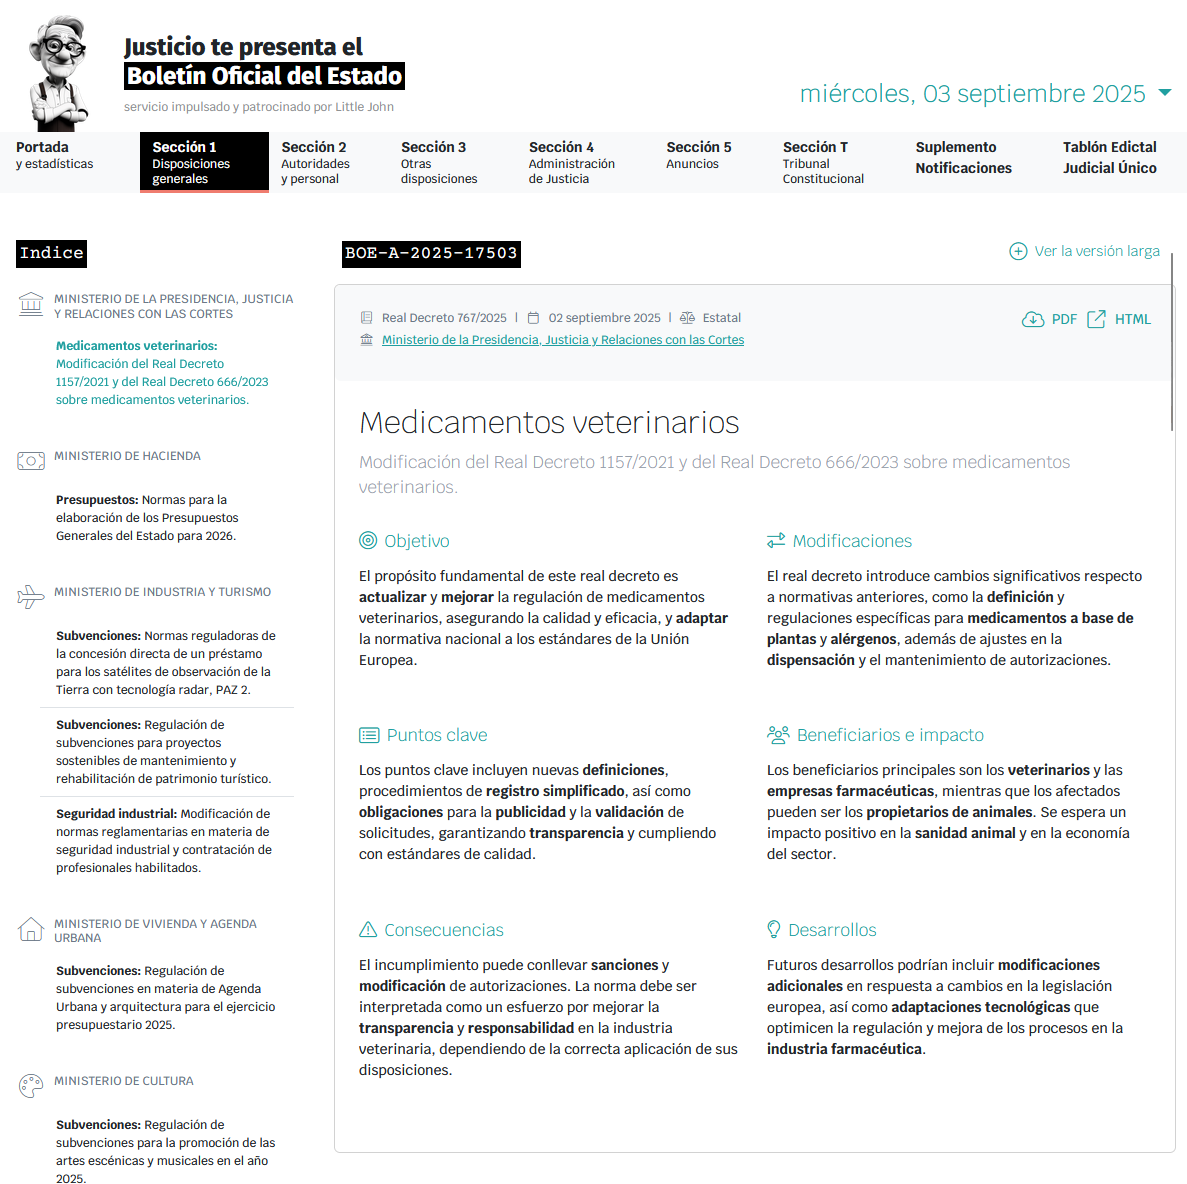
\includegraphics[width=1\textwidth]{imagenes/0160_justicio.png}
	    		\caption{Interfaz de Justicio en el BOE del día 3 de septiembre de 2025 \cite{0060_justicio}}
	    		\label{fig:0160_justicio}
	    	\end{figure} 
	    	
	    	\noindent Con esta evolución, Justicio no solo se ha consolidado como un ejemplo de aplicación práctica de RAG en el ámbito jurídico, sino que también ha logrado democratizar el acceso a la legislación española, transformando un recurso indispensable pero históricamente poco usable como el BOE en una herramienta realmente útil para profesionales y ciudadanos.
	    
	    \subsection{Conclusión sobre las aplicaciones alternativas}
	    
	    	En síntesis, proyectos como \textit{Ajuda Dana} y \textit{TuCocheDana} evidencian la capacidad de la tecnología para ofrecer soluciones útiles en situaciones de emergencia, mientras que \textit{Justicio} demuestra la aplicabilidad del enfoque RAG para hacer más accesible e interpretable la información contenida en el BOE. 
	    	
	    	\noindent En este contexto, el presente trabajo se sitúa en la misma línea, al proponer un sistema RAG aplicado a la documentación del BOE relativa a la DANA, con el fin de mejorar su comprensión y convertir un recurso jurídico denso en una herramienta práctica para la ciudadanía en momentos de crisis.
	    	
    \section{Métodos de evaluación de nuestro RAG}
    \label{2_metods_eva}

        En esta sección se describen las distintas técnicas y configuraciones que utilizaremos para evaluar nuestro sistema RAG. La evaluación se llevará a cabo mediante la combinación de diferentes procesos que afectan tanto a la recuperación de información como a la generación de respuestas. Para finalizar, evaluaremos diversas métricas con las que obtendremos el valor de calidad de los resultados.

        \noindent El conjunto de datos utilizado se almacena en forma de documentos en una base de datos vectorial \textbf{Chroma}, donde cada documento esta pre-procesado y segmentado en fragmentos de \textbf{512} y \textbf{1024} términos respectivamente. Esta decisión se ha tomado para evaluar la granularidad del contenido indexado y la relevancia de los documentos recuperados (enfoque \textit{Naive RAG}) \cite{gao2024retrievalaugmentedgenerationlargelanguage}, asi como la calidad del contexto aportado al modelo generativo.

        \noindent Paralelamente, se ha evaluado el impacto del \textbf{re-ranking} (enfoque \textit{Advanced RAG}) \cite{gao2024retrievalaugmentedgenerationlargelanguage} como paso posterior a la recuperación. Este proceso consiste en el reordenamiento de los documentos recuperados en primera instancia a través de un modelo de recuperación adicional. En nuestro caso usaremos el modelo \textbf{BAAI/bge-reranker-large} disponible en \textbf{HuggingFace} \cite{0036_bge_reranker}, que soporta documentos de más longitud, escritos en más idiomas (a parte del inglés) y a priori, logrará mejores resultados.

        \noindent En las siguiente sub-secciones, listaremos el resto de técnicas usadas para la evaluación del sistema RAG.

        \subsection{Estrategias de búsqueda usadas}

            Se han considerado varias estrategias de búsqueda a la hora de recuperar los documentos más relevantes de la base datos:
    
            \begin{itemize}
                \item \textbf{Similarity}: búsqueda por similitud mediante la distancia coseno en los embeddings.
                \item \textbf{Maximal Marginal Relevance (MMR)}: método usado para recuperar documentos que son a la vez relevante para consulta y diversos entre sí. Este enfoque ayuda a reducir la redundancia e incrementan las aspectos que son cubiertos en los documentos seleccionados \cite{0023_mmr}.
                \item \textbf{TF-IDF y BM25}: métodos clásicos basados en la frecuencia de los términos. TF-IDF se basa en la frecuencia y rareza de los términos del corpus, mientras que BM25 ajusta estos valores dependiendo del tamaño documento.
                \item \textbf{Grafo}: técnica que combina la búsqueda por similitud con relaciones semánticas obtenidas a través de los metadatos de los documentos \cite{peng2024graphretrievalaugmentedgenerationsurvey}. 
            \end{itemize}

        \subsection{Embeddings usados}

            Los embeddings utilizados para indexar y recuperar documentos incluyen los siguiente modelos pre-entrenados:

            \begin{itemize}
                \item \textbf{nomic-embed-text}: Modelo de código abierto entrenado en inglés. Es útil para clasificación, búsqueda y análisis semántico.
                \item \textbf{bge-m3}: Modelo multilingüe con más de cien idiomas. Optimizado para recuperación densa, escasa y multivectorial.
                \item \textbf{snowflake-artic-embed2}: Evolución del modelo anterior de Snowflake, con rendimiento similar a bge-m3. Es también multilingüe.
                \item \textbf{jina-embeddings-v2-base-es}: Biligüe español-inglés, ideal para realizar tareas en español: búsqueda, clasificación, etc.
                \item \textbf{text-embedding-3-small}: Versión mejorada del modelo anterior \textit{text-embedding-ada-002}, modelos pertenecientes a \textbf{OpenAI}.
            \end{itemize}

            \noindent Todos estos modelos están disponibles mediante la plataforma \textbf{Ollama}, exceptuando el último.

        \subsection{LLMs usados}

            Los modelos de lenguaje empleados son los siguientes.

            \begin{itemize}
                \item \textbf{llama3.2:} Modelo perteneciente a Meta de 3B de parámetros. Proporcionado localmente y de forma gratuita por Ollama.
                \item \textbf{mistral-small:} Versión 3.2 perteneciente a Mistral AI, cuenta con 24B de parámetros. Usado a través de la API gratuita de Mistral AI.
                \item \textbf{gpt-4.1:} Nuevo modelo perteneciente a OpenAI. De pago y disponible a través de clave API de OpenAI.
            \end{itemize}

        \subsection{Métricas de evaluación usadas}

            Para finalizar, presentaremos las métricas que se encargarán de medir la calidad de las respuestas de nuestro sistema RAG:

            \begin{itemize}
                \item \textbf{Accuracy}: Evalúa la precisión de la respuesta generada en comparación a la respuesta esperada.
                \item \textbf{Faithfulness}: Evalúa si la respuesta usa la información de los documentos recuperados.
                \item \textbf{Groundness}: Evalúa la capacidad del modelo de apoyar sus respuestas en las evidencias de los documentos recuperados.
                \item \textbf{Relevance}: Evalúa la relevancia de los documentos recuperados para responder a la pregunta.
            \end{itemize}

            \noindent Estas métricas evaluaran nuestro RAG a través de un dataset de preguntas generado a partir de los documentos de la fuente de conocimiento.